\label{sec:2_background_theory}


% Broader picture
\section{Artificial Intelligence}

% Short intro
\gls{ai} is both a research topic and a group of approaches aimed at giving computer programs the most intelligent possible approach to solving a given task. In academia, it became a research topic in 1956 after a conference called the Summer Research Project on Artificial Intelligence, which was hosted by John McCarthy and Marvin Minsky, which is considered to be where the term originated and is often credited to McCarthy \cite{mccarthyProposalDartmouthSummer2006, andresenJohnMcCarthyFather2002}. Since this first conference, the field has evolved with the help of an interdisciplinary environment of computer science, mathematics, statistics, psychology, neurology, and linguistics.

% What this section is about
Overall, this section of the thesis provides a brief overview of the history of AI and sheds light on the importance of the field in modern society. It forms the basis for the further discussion of relevant AI concepts in the following sections of this work.

Throughout history, humans have had the desire to wield the power of creating artificial creatures. The concept of artificial beings that are able to observe, evaluate and react to their surroundings can be dated back to the story of Talos in Greek mythology \cite{universityAncientMythsReveal2019}. The concept has since been featured in countless fiction novels and movies, such as Frankenstein, R.U.R, HAL9000, and Metropolis \cite{shelleyFrankensteinModernPrometheus1992, capekRossumUniversalRobots, kubrick2001SpaceOdyssey1969, langMetropolis1927a}. 

Humanity has since taken the dream of artificial beings with consciousness from the realm of fiction and driven the evolution of \gls{ai} as a research field forward with impressive results. 
AI has become an integral part of people's everyday lives, fueling advances in science and technology, including social media, computational photography, voice assistants, and chatbots \cite{barbastathisUseDeepLearning, hoyAlexaSiriCortana2018, biswasRoleChatGPT2023}. Doctors can now use artificial intelligence to interpret medical images, and artists are using AI to create new art \cite{wangMachineLearningRadiology2012, thrallArtificialIntelligenceMachine2018}.


\subsection{A Short History of AI}
% Alan Turing 
The origins of modern AI can be traced back to the 1940s and 1950s, when pioneers such as Alan Turing and John McCarthy laid the foundations for today's AI research methods. 

Alan Turing was a British mathematician and pioneer of computer science, and he is most notably known for his contributions to the development of modern computer theory. In 1936, Turing presented his theory of computation, which proposed a system later coined as a Turing machine, which is an abstract machine that manipulates a strip of tape using only simple rules. Despite its limited rules, they can be combined to interpret any proposed computer algorithm. The theory was revolutionary at the time and laid the foundation for the development of modern computers and later became known as the Church-Turing thesis \cite{turingSystemsLogicBased1938, churchUnsolvableProblemElementary1936}. 

One of the first to use Turing's theories in practice was McCullough and Pitts and their formal design of artificial neurons in 1943 \cite{mccullochLogicalCalculusIdeas1943, piccininiFirstComputationalTheory2020}, which was the first step towards the method now known as the perceptron. In 1950, Turing proposed a behavioral test, originally called the imitation game and later named the Turing test. This behavioral test was set up so that a human would speak to two separate entities, the human judge knowing that one was another human and the other a machine. Then the human would talk to those two participants, not knowing whether the responder was the human or the machine, and then try to decide who the machine was. The computer would pass the Turing test if the human judge could not distinguish between human and computer. This test is relevant today with tools such as ChatGPT \cite{ChatGPT}, where the boundary between human and machine-produced natural language disappears. Turing's work laid the foundation for modern computers and artificial intelligence. His ideas are still relevant today, and his impact on the field of computer science cannot be overstated. The Church-Turing thesis, in particular, had a significant impact on the research field of studying computers and giving an understanding of the limitations of computer systems. Turing's work also laid the foundation for the development of artificial neural networks and their use in machine learning.

The research field of artificial intelligence has gone through several ups and downs over the years. These ups and downs have mostly been caused by increased popularity and interest in founding new technologies in the field, followed by disappointment when the development didn't deliver the desired results. Disappointment led to cuts in funding, which stagnated development. The AI industry has experienced two significant cycles of reduced interest, often referred to as the two AI winters. The first AI winter was in the late 1970s, and the second was in the late 80s to early 90s \cite{floridiAIItsNew2020}. Since the beginning of 2012, interest in AI has increased, driven in particular by advances in machine learning, deep learning, and increased computing resources. With the advent of deep learning and big data, AI has seen a resurgence, and unprecedented advances have been made in the field in recent years. This has led to the development of intelligent systems that can take on a variety of tasks that were once thought to be an exclusive domain of humans, such as driving cars and interpreting images. 

Artificial intelligence can be divided into two main paradigms that take different approaches to achieving artificial models. The two paradigms are named symbolic and connectionist \gls{ai}.


% Symbolic artificial intelligence
\subsubsection{Symbolic Artificial Intelligence}


Symbolic Artificial Intelligence refers to a collection of AI methods based on high-level symbolic representation of problems. It is also known as rule-based AI, classic AI, and good old-fashioned AI (GOFA) \cite{haugelandArtificialIntelligenceVery1989}. 

In the period between the 1950s and mid-1990s, symbolic representation was seen as dominant over the other main representation, connectionism, which will be discussed in the next sub-chapter. This was because symbolic representation came closer to the thought human way of learning symbolic representations rather than analyzing neuron activation in the brain and therefore had an advantage over connections \cite{garneloReconcilingDeepLearning2019}. 
The goal was to provide machines/computer code with human knowledge and patterns of action by defining rules in programs. The main idea behind symbolic AI is to define a high-level symbolic representation that creates the building blocks for the intelligence of the program. In addition to these pre-programmed rules, an expert system is used, which then checks which rules are fulfilled and makes a decision on this basis.

The advantage of symbolic AI is that because of the pre-programmed rules, it is more transparent about what underlies the decisions, and, given the same assumptions, the same result is obtained every time. Because of the rule-based nature of the algorithms, they work well even on data with little variation. They also work well for datasets with few examples because programmers can use a priori knowledge of the problem when defining the rules.

Symbolic AI has disadvantages in that irregular variations cannot be accounted for other than creating new and additional rules to cover all variants that may be encountered. This is a disadvantage in systems that process data from the real world, as they often contain large variations. It is, therefore, often practically impossible to write rules to cover all variations unless the task is severe and well-defined.


% Connectionist artificial intelligence
\subsubsection{Connectionist Artificial Intelligence}
Despite developing in the background of Symbolic AI during the first decades of its academic history, new methods have made connectionist AI remarkably popular in recent times. Connectionism is based on the idea that the interconnection of several small nodes, which learn over time, forms intelligent judgment systems. This approach is often compared to how the brain works, as it is connected by a network of neurons. The most well-known example of such a method is the artificial neural network, which is built up of many processing nodes, often called perceptions \cite{mccullochLogicalCalculusIdeas1943}.

The perceptron is inspired by biology and mimics a biological neuron. This perceptron takes data as input, weights it according to its learned importance, and then uses a transfer function to provide an output. These small artificial neurons are connected in layers and learn from sample data fed into the model. The model learns by adjusting weights that define the importance of input to make a correct assessment.

Since 2012, models that can train on increasingly large datasets have improved significantly, in large part due to advances in computational power. Connectionism has given a new boost to AI as a field and tool in real-world applications, and they are constantly being renewed to solve new problems.

The main benefit of connectionism is that the model can learn more complex relationships than symbolic \gls{ai} since the weights in the neurons can be updated as new examples are trained. This allows the method to extract information from datasets with large variations between individual samples.

The main downside, however, is that it's often difficult for humans to gain insight into the formation of judgments, as the process learns by adjusting weights in each of the many neurons. The models, therefore, can learn connected structures that humans would not pick up. Another disadvantage of these models is that they often become more accurate with more data and more complex model structures, making accurate models harder to interpret. Because of the difference in how humans reason and some deep artificial networks learn, new fields of research like \gls{xai} try to make models more transparent and understandable.


    % Combining these two representations
    \subsubsection{Combination of Symbolic and Connectionist AI}
    With the rapidly growing market and the development of new \gls{ai} tools, there is increasing pressure to make connectionist models more transparent by combining symbolic and connectionist \gls{ai}, known as neuro-symbolic AI \cite{valiantKnowledgeInfusionPursuit2008}. The advantage of combining these two paradigms is that these combined models utilize the properties of connectionist models to train on large datasets with significant variations, in addition to learning symbolic representations of the dataset, making it easier for humans to understand the basis for the model's decisions.

    In the book Thinking Fast and Slow by Daniel Kahneman \cite{kahnemanThinkingFastSlow2013}, a model of human thinking is discussed. It is proposed that human thinking is composed of two systems, one fast and intuitive and the other a slower, more deliberate system. The book argues that the symbiosis of these two systems makes human thinking more robust and reliable. In this context, the neuro-symbolic AI comprises a fast symbolic pattern recognition system, and a connectionist deep learning model takes care of the more deliberate reasoning.  
    
    This type of model can train on large datasets of e.g. images while learning from question-and-answer pairs to become familiar with linguistic symbols such as colors and shapes. The hope is that this will lead to a more general understanding from the model's perspective by learning multimodally and being able to learn variations in the dataset using fewer examples while being somewhat transparent.
    
    The integration of models across modalities is further explored in this work. It is an interesting research area where the combination of connectionist and symbolic approaches can make AI models more transparent, easier to understand, and more meaningful to work without sacrificing accuracy and applicability.


    \subsection{Machine Learning}

    The field of artificial intelligence includes a subgroup subset known as machine learning. Because these two groups are often conflated in the media, it is reasonable makes sense to define machine learning as a subset of AI, although some argue that machine learning has diverged from AI, with overlaps, overlaps as illustrated in Figure \ref{fig:ai_ml_dnn_argue} \cite{raschkaChapterIntroductionMachine2020}. This thesis treats \gls{ml} as a sub-field of AI, as shown in Figure \ref{fig:ai_ml_dnn}.


    \begin{figure}[htb]
        \centering
        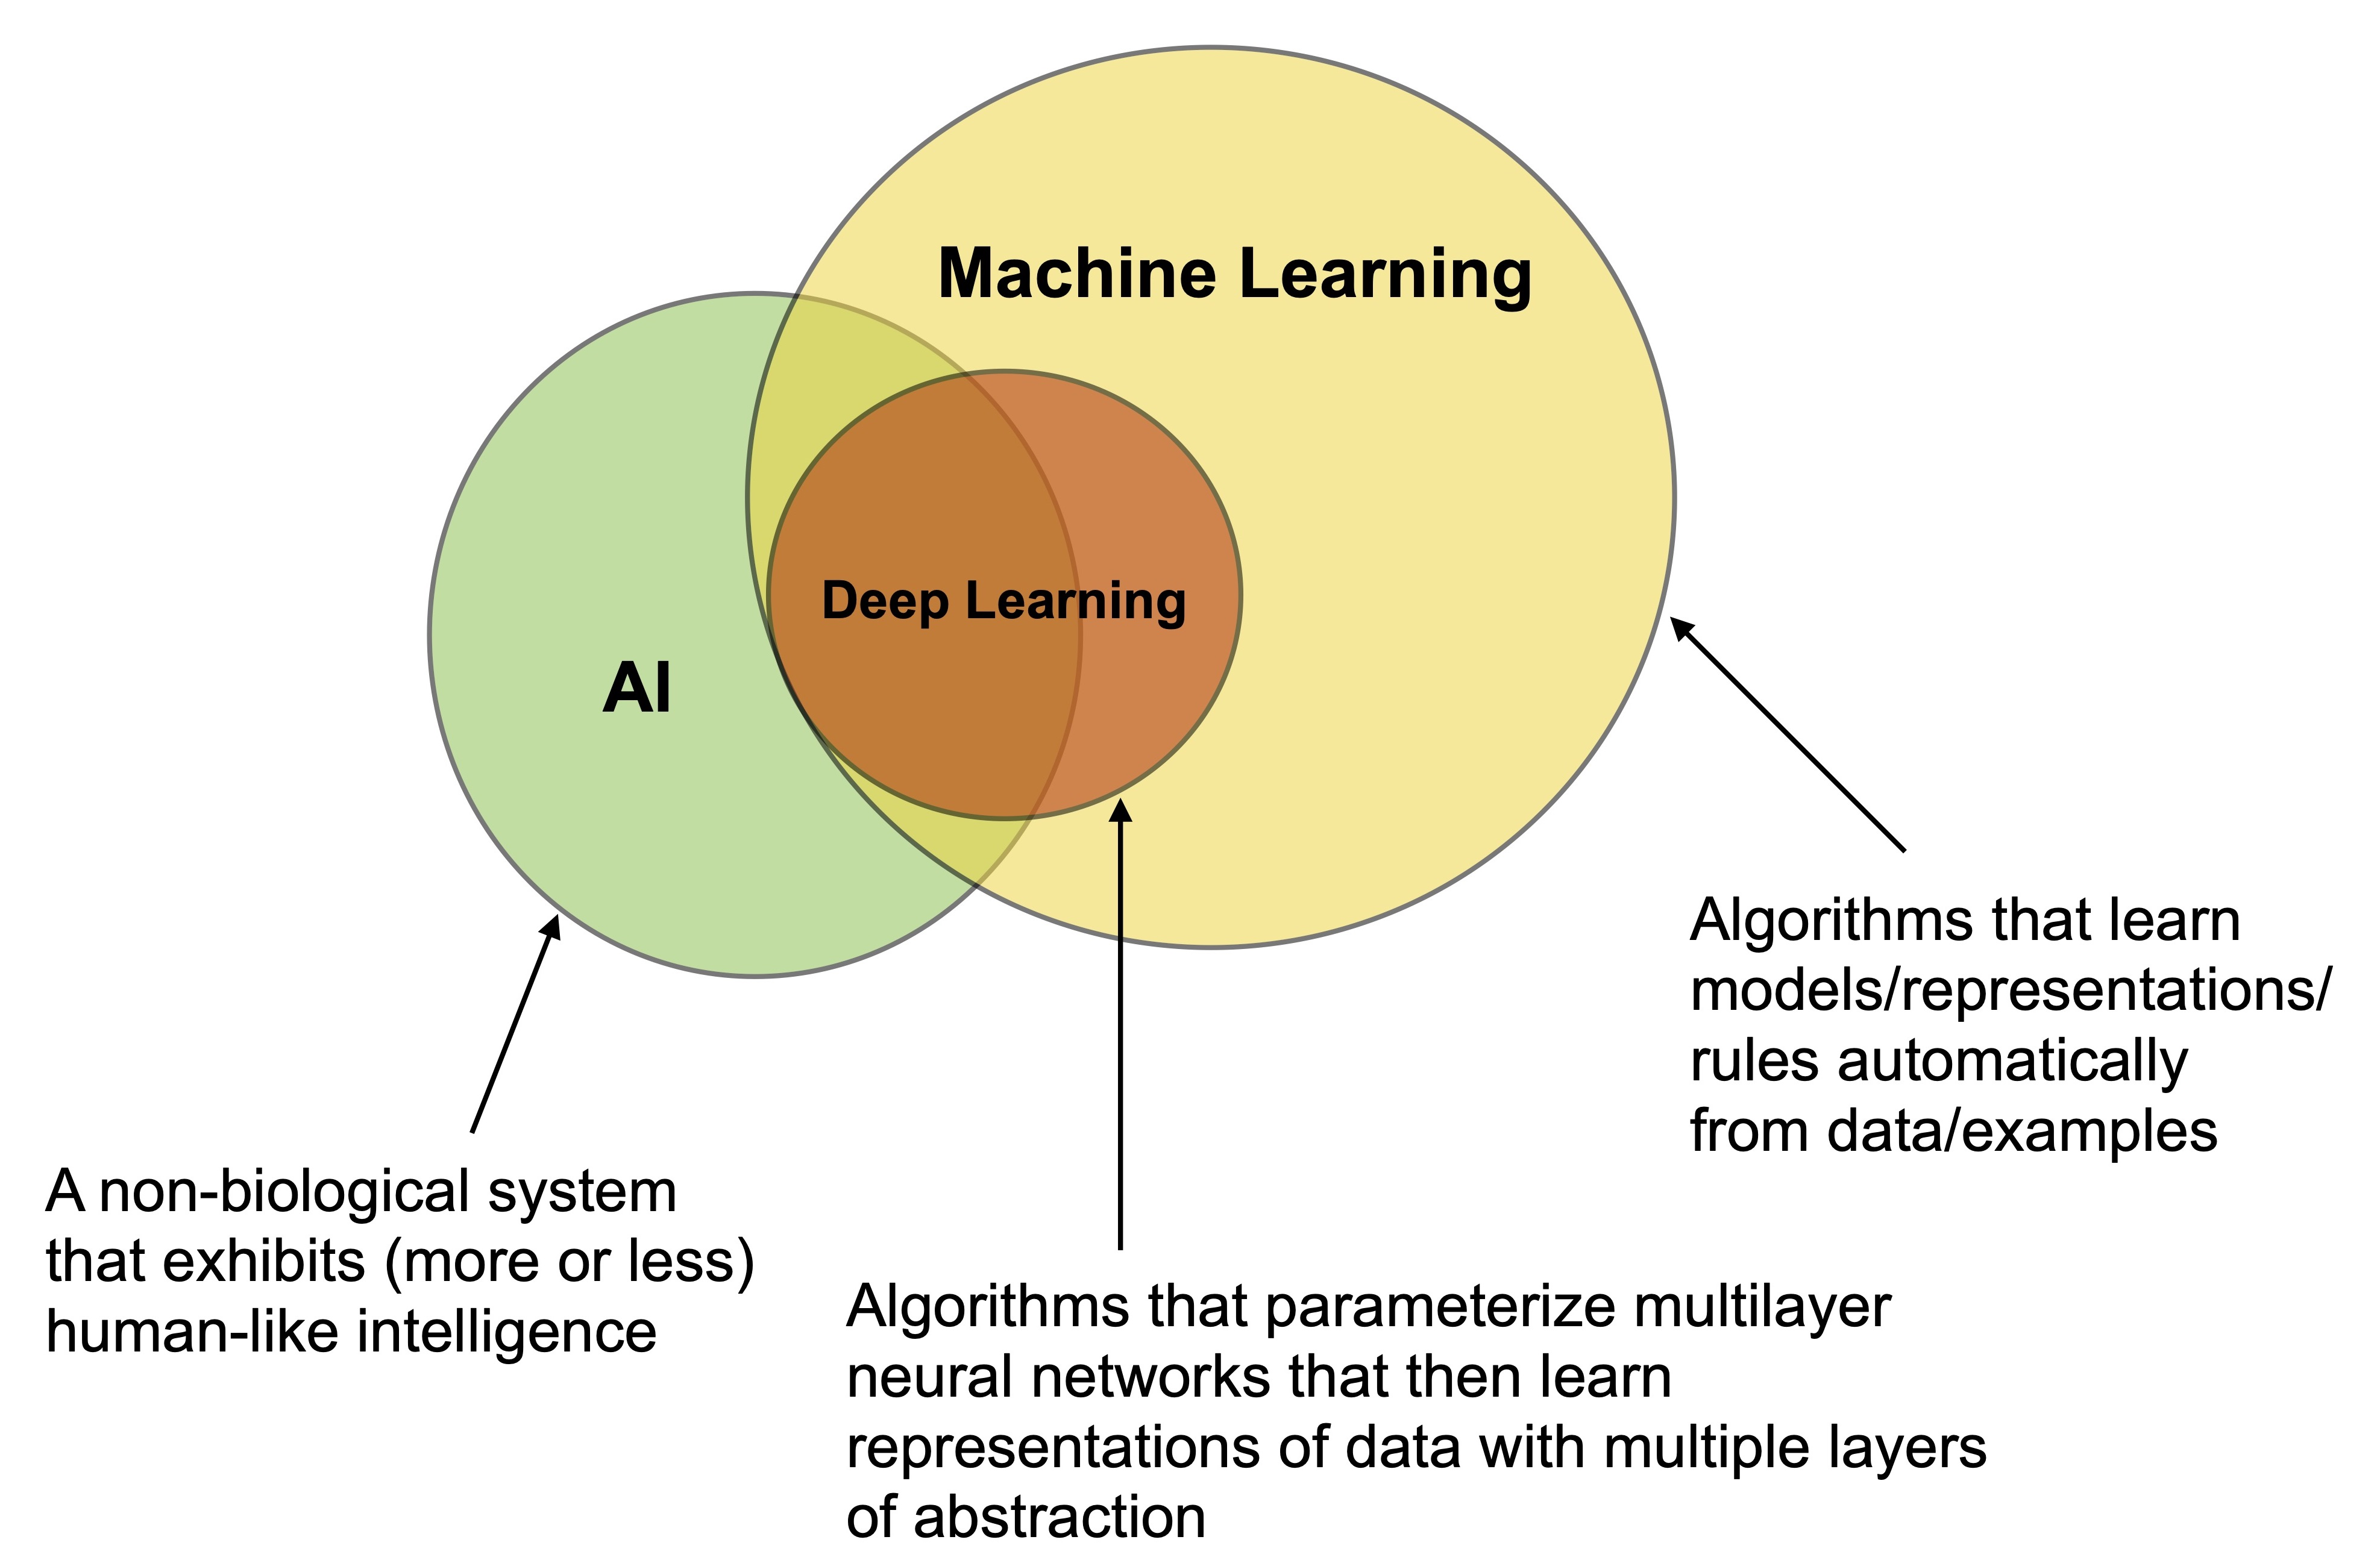
\includegraphics[width=\linewidth]{images/ai_ml_dnn_argue.jpeg}
        \caption[Overview of an alternative structure for \gls{ai}, \gls{ml}, and deep learning. This structure argues that AI is the pursuit of developing non-biological systems with human-like intelligence and can be achieved with methods that do not use machine learning or deep learning, such as symbolic representations in a shallow architecture.]{Overview of an alternative structure for \gls{ai}, \gls{ml}, and deep learning. This structure argues that AI is the pursuit of developing non-biological systems with human-like intelligence and can be achieved with methods that do not use machine learning or deep learning, such as symbolic representations in a shallow architecture. This representation is not de facto and is not used in this work.\\Figure credit: Raschka \cite{raschkaChapterIntroductionMachine2020}}
        \label{fig:ai_ml_dnn_argue}
    \end{figure} 

    \begin{figure}[htb]
        \centering
        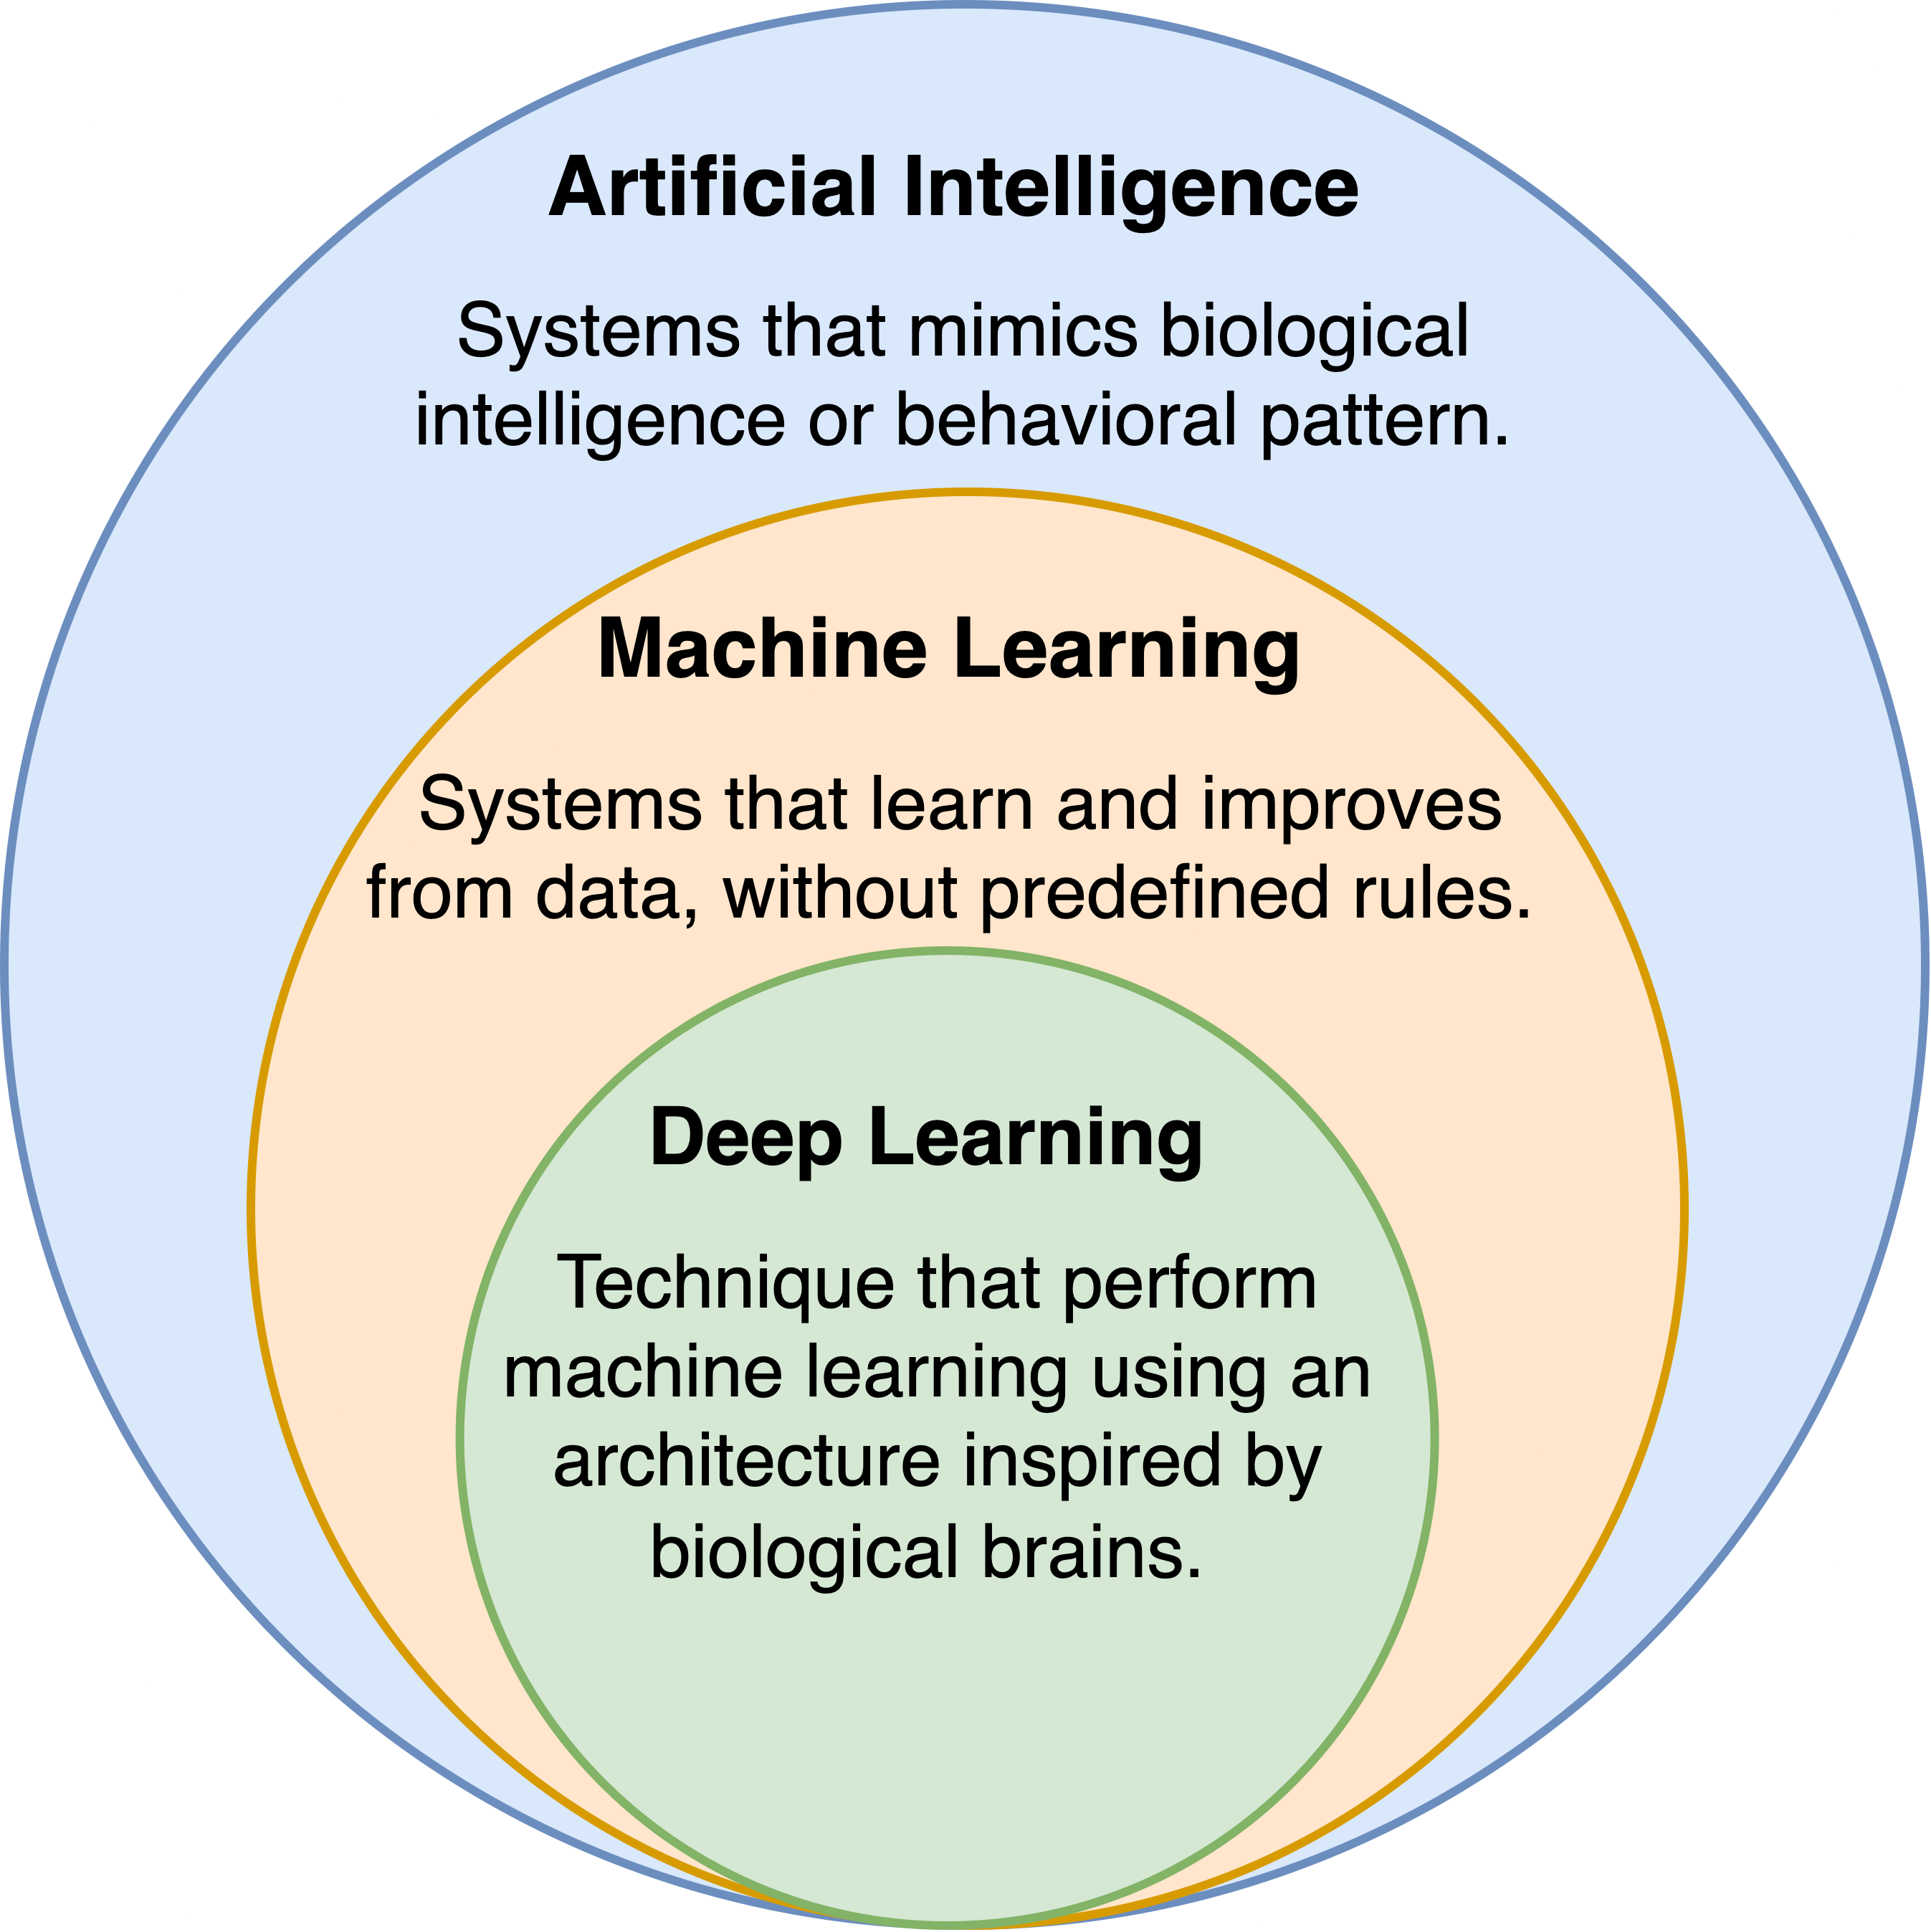
\includegraphics[width=9cm]{images/ai_ml_dnn.png}
        \caption[Overview of the structure between artificial intelligence, machine learning, and deep learning. This is the structure used in this thesis.]{Overview of the structure between artificial intelligence, machine learning, and deep learning. This is the structure used in this thesis. Figure by the author.}
        \label{fig:ai_ml_dnn}
    \end{figure} 

    Machine learning is often broken down into three sub-areas, which are discussed and explained in this sub-section, explaining how they work, under what circumstances each sub-area can be used to advantage, and the challenges each branch faces are highlighted.

        \subsubsection{Supervised Learning}

        The first category within machine learning is known as supervised learning. This method is conceptually similar to using flashcards for memorization.
        The participant draws a card and reads the question while keeping the answer hidden. Only after the participant answers the question the correct answer can be revealed. This is, in essence, the same approach used in supervised learning.
        
        
        In supervised learning, a dataset with pre-labeled examples, also known as a fully labeled dataset, is used to train algorithms to predict labeling for unlabeled input data. This is typically accomplished by training on a larger dataset with labels for each input, passing the input through a network, and using the label to inform the algorithm what the input data should be labeled as. In this way, the method learns the relationship between the input and the correct label. The method learns these correlations by adjusting the weights within the network to produce a result that is as close as possible to the true label.
        
        Since the ground truth label is known for each entry in the dataset, the model's output is compared to this ground truth label, and the accuracy of the similarity between these two is measured using a loss function. Weights are adjusted using a technique called backpropagation to minimize this loss, and training continues until the weights are appropriately adjusted to achieve a satisfactorily low loss. These weights are then used later when testing real-world inputs, for which ground truth is often unavailable and must be estimated.
        
        Within supervised learning, there are two main subcategories: classification and regression. 
        
        Classification is a method used when the output variable belongs to a category, such as a color or an object, or to indicate the probability that an input belongs to one or more categories. Classification either predicts categorical class labels or classifies data by building a model. A typical classification method can be used to sort emails into spam or not spam or to identify the bird species in an image. Classification models can include methods such as neural networks, \gls{svm}, \gls{knn} \cite{fixDiscriminatoryAnalysisNonparametric1989, coverNearestNeighborPattern1967}, random forest, decision trees, one-vs-rest, and naive Bayes. Section \ref{sec:2_background_theory_deep_learning_and_neural_networks} will go into more detail about neural networks, as this is a very central method of machine learning and is relevant to this work, as it is used later in this thesis by the first proposed architecture in Section \ref{sec3:proposed_architecture}.
        
        The second approach within supervised learning is called regression. This method is used when the output should be a real or continuous value. Regression is used to find the correlation between dependent and independent variables. There are many different models within regression, such as linear regression, logistic regression, and polynomial regression. It is common to use hyperplanes that fit the available data. Regression is often used to make forecasts based on past data, e.g., estimating real estate prices for an area or salary growth.


        \subsubsection{Unsupervised Learning}

        Unsupervised learning is a technique that uses raw data from a given dataset to identify patterns and relationships in unlabeled data, facilitating the grouping of each item into appropriate clusters. The essence of this approach is that it can autonomously analyze and group data without requiring human intervention to pre-label the data. Therefore, it is well suited for use in data analysis, image recognition, and image segmentation.

        
        
        The main grouping models used in unsupervised learning are clustering, association, and dimension reduction. Clustering aims to divide raw data into groups or clusters based on similar characteristics. An example of a cluster split is shown in Figure \ref{fig:knn}, demonstrated by the \gls{knn} method. Association rules, on the other hand, are a rule-based approach that attempts to uncover relationships between variables in a dataset. These associations can, for example, be used in recommendation models, where companies can identify correlations between customers who purchase different items and use this knowledge to suggest similar products to new customers.

        \begin{figure}[htb]
         \centerline{
             \begin{subfigure}[b]{0.37\textwidth}
                 \centering
                 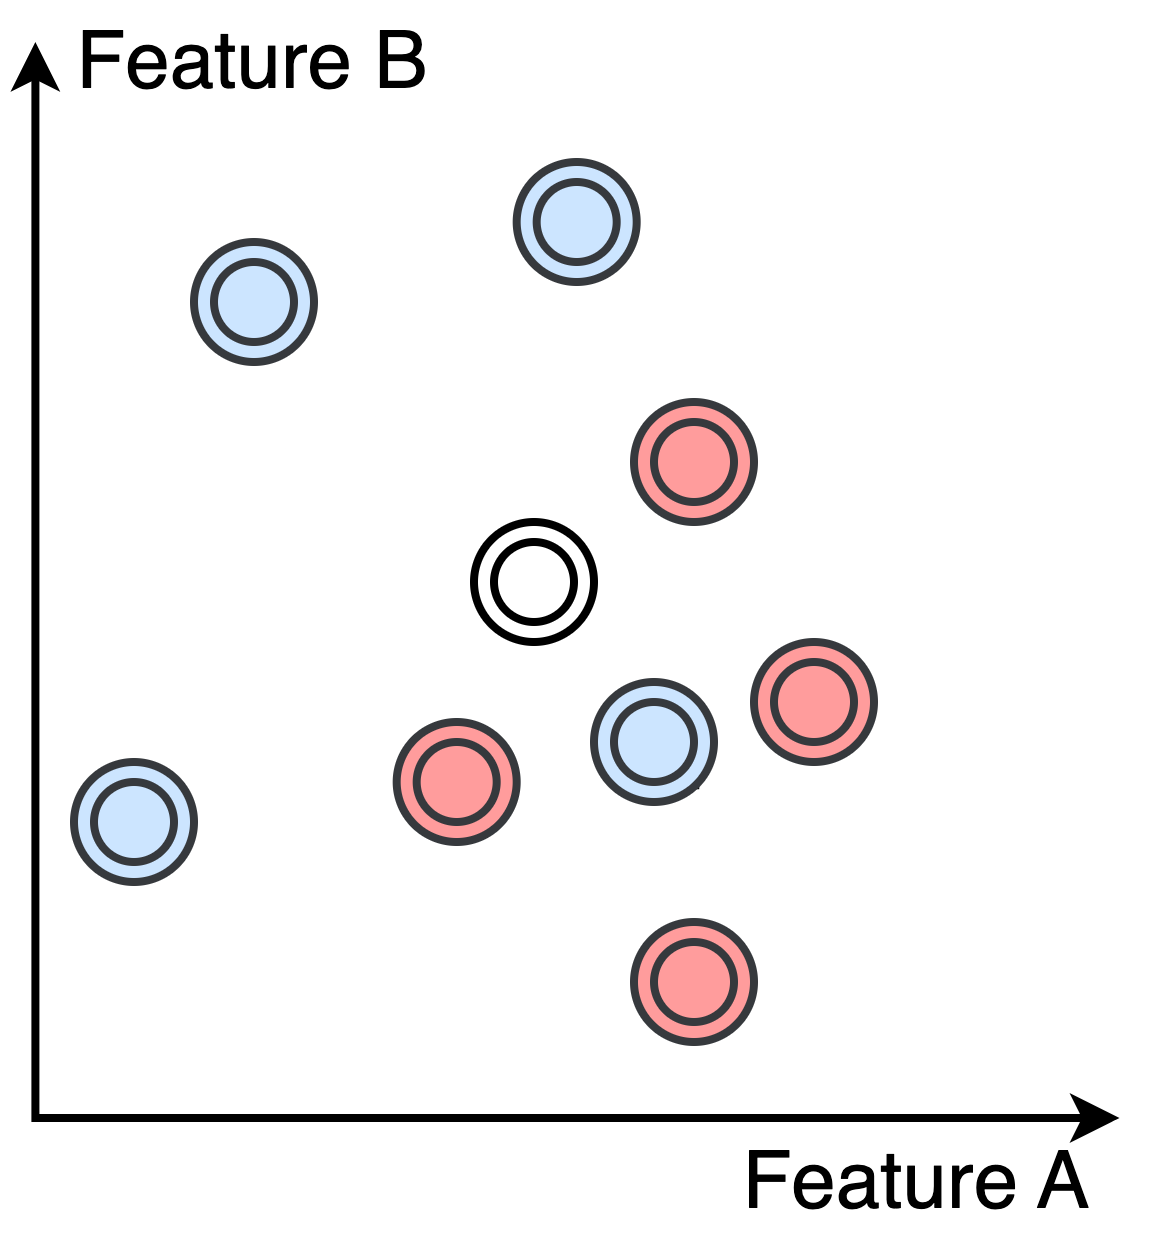
\includegraphics[width=\textwidth]{images/knn_1.png}
                 \caption{Samples are distributed in a feature space. The colors represent class, and the white is a new sample. A new sample will be classified based on neighboring samples.}
                 
             \end{subfigure}
             \hspace{0.015\textwidth}
             \begin{subfigure}[b]{0.37\textwidth}
                 \centering
                 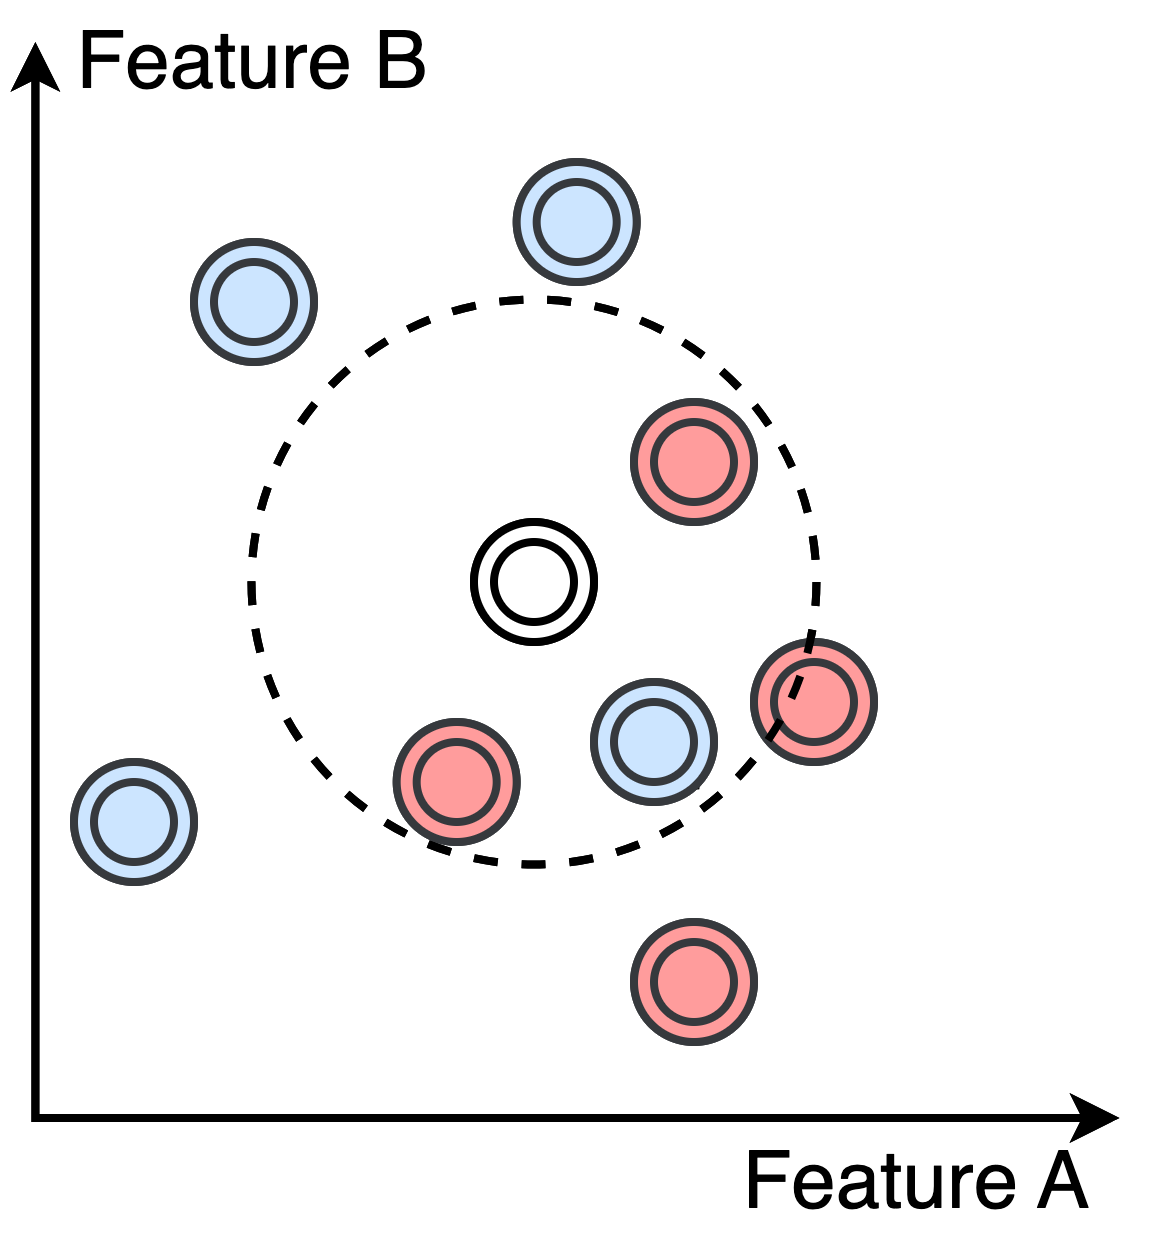
\includegraphics[width=\textwidth]{images/knn_2.png}
                 \caption{The new sample checks the nearest neighboring samples. In a circumference, noted with a dotted circle, the 4 closest neighboring samples are found.}
                
             \end{subfigure}
             \hspace{0.015\textwidth}
             \begin{subfigure}[b]{0.37\textwidth}
                 \centering
                 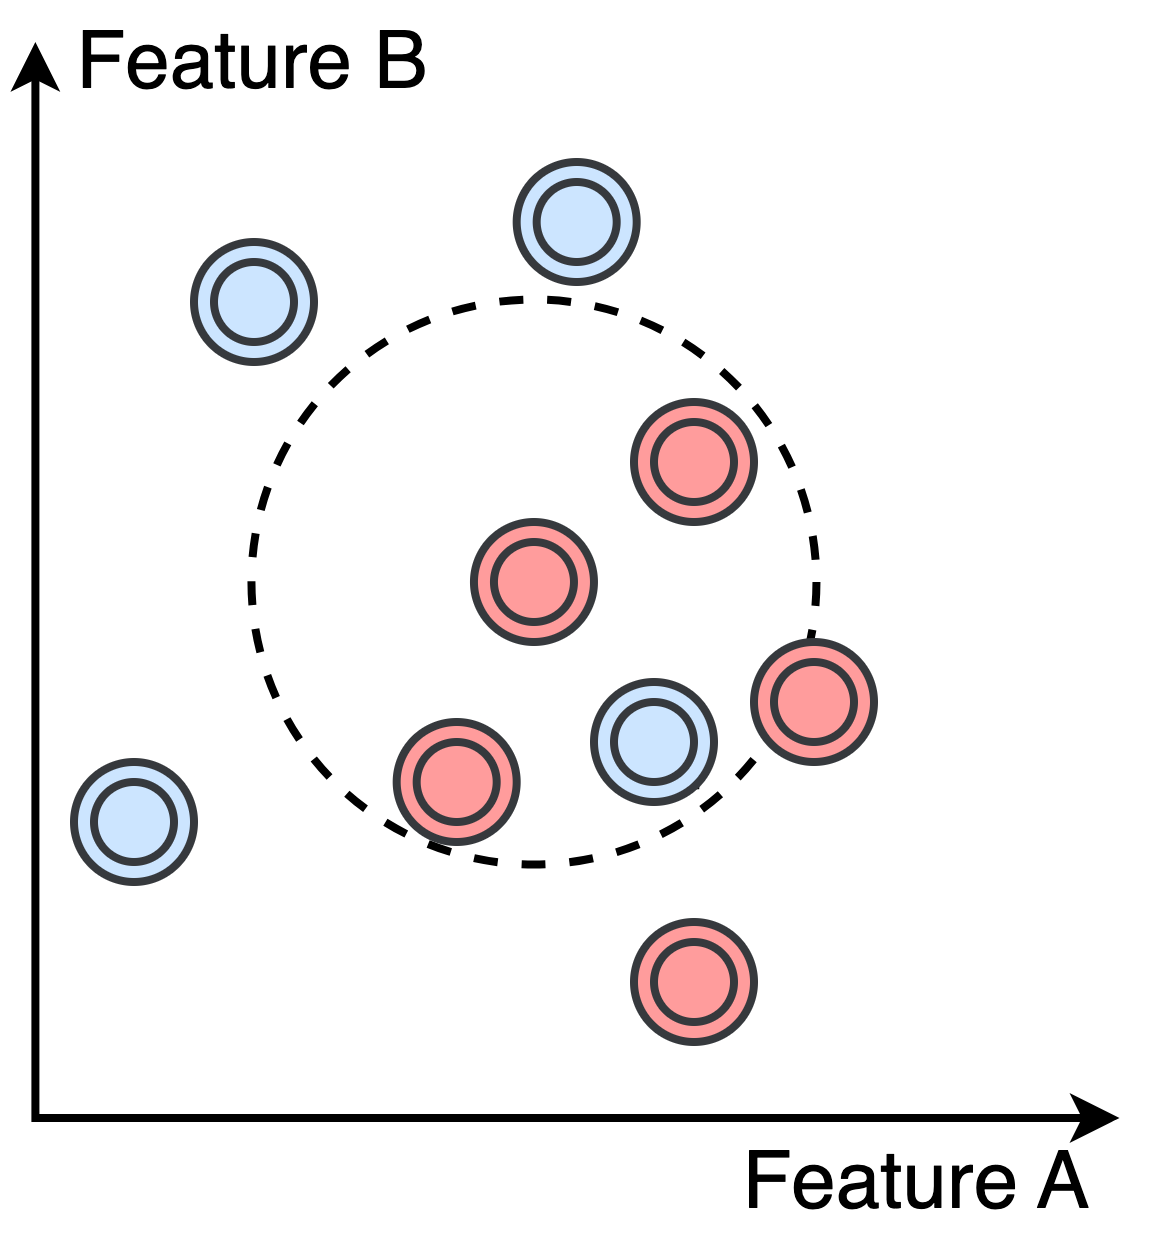
\includegraphics[width=\textwidth]{images/knn_3.png}
                 \caption{The classes of the 4 closest samples are counted, and the majority class is chosen. Of the 4 samples, one is blue, and three are red. The new sample is therefore classified as red.} 
             \end{subfigure}
             }
            \caption{Example of how the clustering algorithm k-Nearest Neighbors computes the class of a new sample. Figure by the author.}
            \label{fig:knn}
        \end{figure}
        
        Dimensionality reduction is a technique for reducing the number of dimensions in a dataset. 
        Although many machine learning methods benefit from additional data, this is not always the case \cite{belkinReconcilingModernMachinelearning2019, nakkiranDeepDoubleDescent2021}. Data samples can often contain insignificant variables or noise, making model training ineffective and making the dataset in practice smaller regarding useful information. This technique can be used to create a dataset containing more distinct features and also visualize and analyze data. When reducing the dimensions of a dataset, the goal is to reduce the number of learnable parameters while maintaining the integrity of the data being processed. Well-known methods for dimension reduction are \gls{pca} and \gls{svd}. More recently, good results have been obtained with deep neural network-derived autoencoders \cite{sakuradaAnomalyDetectionUsing2014}. Autoencoders can compress data fed to them and produce a representation or encoding that retains much of the underlying data, but the dimensions are significantly reduced.
        To retrieve this data after encoding, a decoder is required to reconstruct the data. Figure \ref{fig:auto_encoder} depicts an autoencoder with an encoder and decoder.

        \begin{figure}[htb]
            \centering
            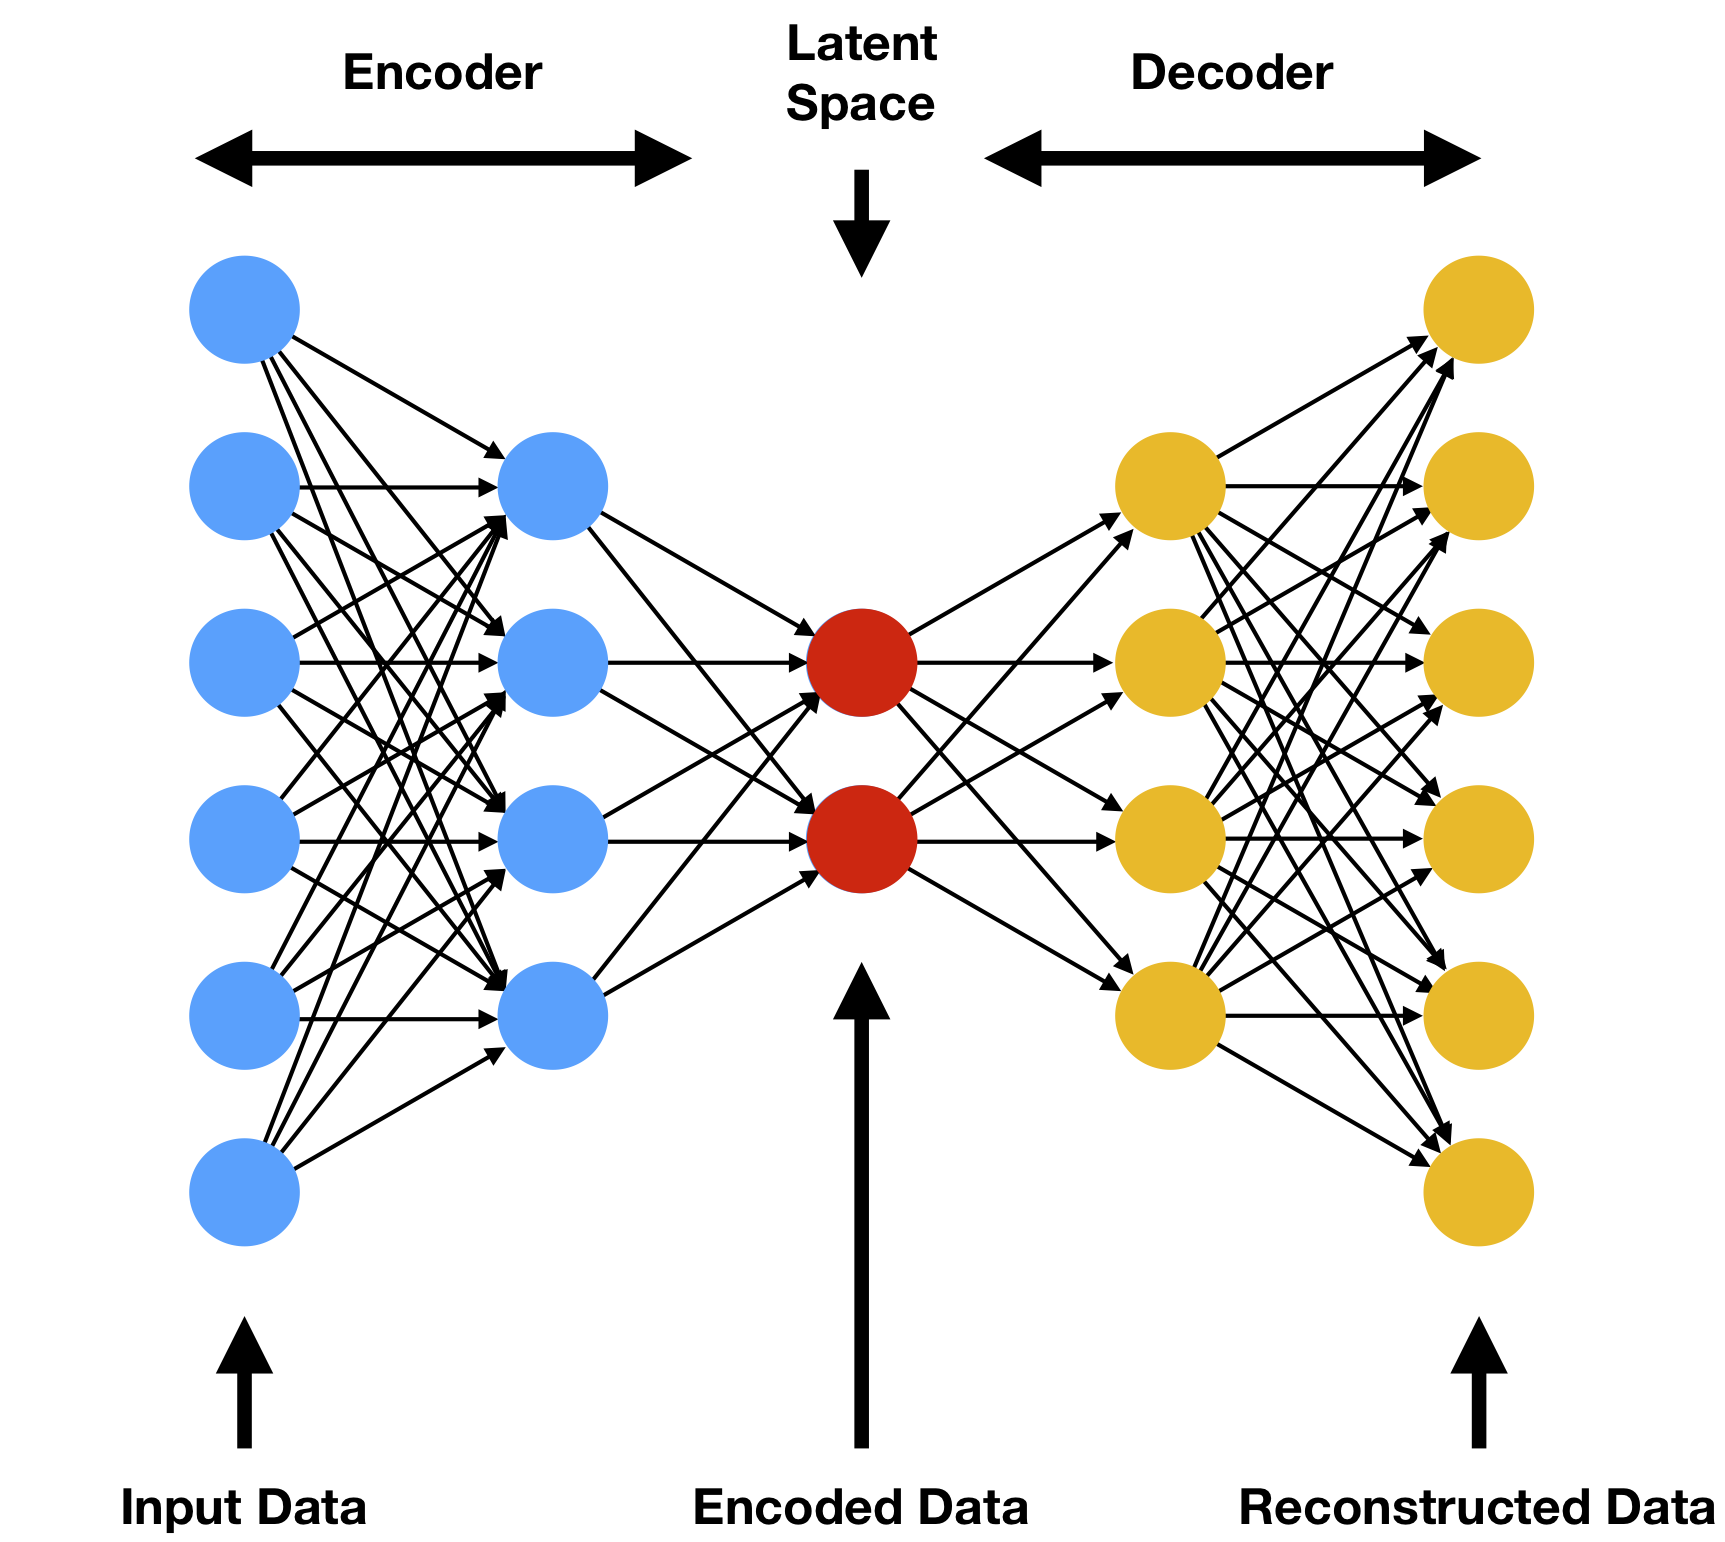
\includegraphics[width=11cm]{images/auto_encoder.png}
            \caption{A diagram of an autoencoder consisting of an encoder and a decoder network. The encoder network maps the input image into a low-dimensional representation, while the decoder network reconstructs the original image from the low-dimensional representation. By minimizing the reconstruction error between input and output, the autoencoder can learn a compressed representation of the input data.\\Figure credit Steven Flores \cite{floresVariationalAutoencodersAre2019}.}
            \label{fig:auto_encoder}
        \end{figure} 
        
        Unsupervised learning has proven useful in computer vision, where it can aid in object recognition, detection, and segmentation, such as in medical datasets. By allowing correlations to be identified and grouped into clusters based on features or traits, unsupervised ML can also be used for anomaly detection, where it can flag atypical data. This method is also often used in recommendation engines, such as those found in online stores, streaming services, or social media.


        \subsubsection{Semi-Supervised Learning and Hybrids}

        % https://en.wikipedia.org/wiki/Semi-Supervised_Learning#Semi-supervised_learning
        % https://en.wikipedia.org/wiki/Active_learning_(machine_learning)
        % https://ai.stanford.edu/blog/weak-supervision/
        % https://medium.com/geekculture/weak-supervision-and-active-learning-352fe8dc7df8
        % https://snorkel.ai/weak-supervision/
        % https://www.youtube.com/watch?v=SS9fvo8mR9Y
        % https://www.youtube.com/watch?v=-cc2RYF37zE

        Supervised learning is often more accurate than unsupervised learning as it can learn from the knowledge provided by humans in the form of labeled data. This approach can also avoid computational complexity since the model does not need to train on irrelevant features for the specific task. However, the downside of supervised learning is that it requires significant human effort beforehand labeling the dataset, which can be time-consuming and costly, particularly when domain experts are required.

        A hybrid solution that aims to leverage the best of both supervised and unsupervised learning is known as semi-supervised learning. This approach can be beneficial when there is too much data to label, either because the dataset is large or the cost of labeling is high. Semi-supervised learning typically assumes that data points close together in feature space share labels or have an underlying correlation factor in a lower dimension (manifold hypothesis/assumption). Methods using semi-supervised learning often achieve higher accuracy than those using only supervised or unsupervised approaches separately because they do not need to discard data that is not labeled and can be trained using a researcher's a priori knowledge of the dataset or possible solution.
        
        Other approaches, such as active learning and weak supervision, can also often be used when a fully labeled dataset is unavailable for training. Active learning is a process in which a model can select input data about which it is unsure and ask a human or other expert for the correct answer. For example, such methods can label large data sets with services such as Amazon Mechanical Turk \cite{AmazonMechanicalTurk}. Samples are selected using a model that attempts to ask for samples believed to have the highest value for further classification. This can be achieved by first asking an expert for a sample from random samples and fitting the model to obtain a decision boundary that separates the classes. After that, the model can iteratively identify examples of high importance since they are near or at this decision boundary. These are the most uncertain examples, making them valuable for the model to identify. Then the model asks the expert for samples near the boundary. The boundary is adjusted again, and the process is repeated until the model fits the data and satisfactorily separates the samples.
        
        Weak supervision is a method that can be applied in situations where it is preferable to have a large number of sufficiently accurate examples rather than a smaller number that are completely correct \cite{hoffmannKnowledgeBasedWeakSupervision2011}. This approach is often implemented by defining some rules or using a knowledge base in advance, which helps the model estimate the probability that an example belongs to a certain category. Weak supervision is often used in conjunction with transfer learning, which involves transferring knowledge from one area to another \cite{wangSimVLMSimpleVisual2022}. Transfer learning has shown promising results because generalizable knowledge of data can often be transferred, eliminating the need to learn from scratch on a new dataset. Transfer learning can be combined with other methods, e.g., supervised learning \cite{zhuangComprehensiveSurveyTransfer2021}.
    
    \subsection{Deep learning and Neural Networks} \label{sec:2_background_theory_deep_learning_and_neural_networks}
    Neural networks, also known as \glspl{ann}, are an ML method inspired by how the biological brain processes information and learns. Essentially, \glspl{ann} approach the goal of extracting information and constructing knowledge by forming a network of artificial neurons that can process input data. These artificial neurons, called perceptrons, are the building blocks of neural networks and are likewise inspired by biological neurons. In this representation, the inputs to the artificial neuron are synapses on the dendrites, the axon hillock inspires the activation function, and the output from the artificial neuron is the biological axon.
    
    The artificial neurons process data by weighting the input data and a predetermined bias before passing it through an activation function, such as a sigmoid or ReLu \cite{dubeyActivationFunctionsDeep2022} that produces the neuron's output. When the output of the activation function exceeds a certain threshold, the neuron is activated and sends data to the next layer. No further data is sent if the output does not exceed the threshold.

    \begin{comment}
    % Remove this
    This processing step of a perceptron can be viewed as a linear regression, as in shown formula ?. However, unlike linear regression, perceptrons in \glspl{ann} are connected in a network, so changes in weights cascade to the next level of perceptrons. A single-layered neural network can therefore be seen as a logistic regression function.
    \end{comment}
    
   \glspl{ann}, often called multi-layer perceptron (MLP), are the cornerstone of deep learning, which refers to \glspl{ann} with more than three layers. The smallest deep network, therefore, has an input layer, two hidden layers in the middle, and an output layer. These middle processing layers are called the hidden layer because it is hidden from the outside, which the input and output layers are not. An example of such a network with two hidden layers is shown in Figure \ref{fig:deep_network} to see. 


    \begin{figure}[htb]
        \centering
        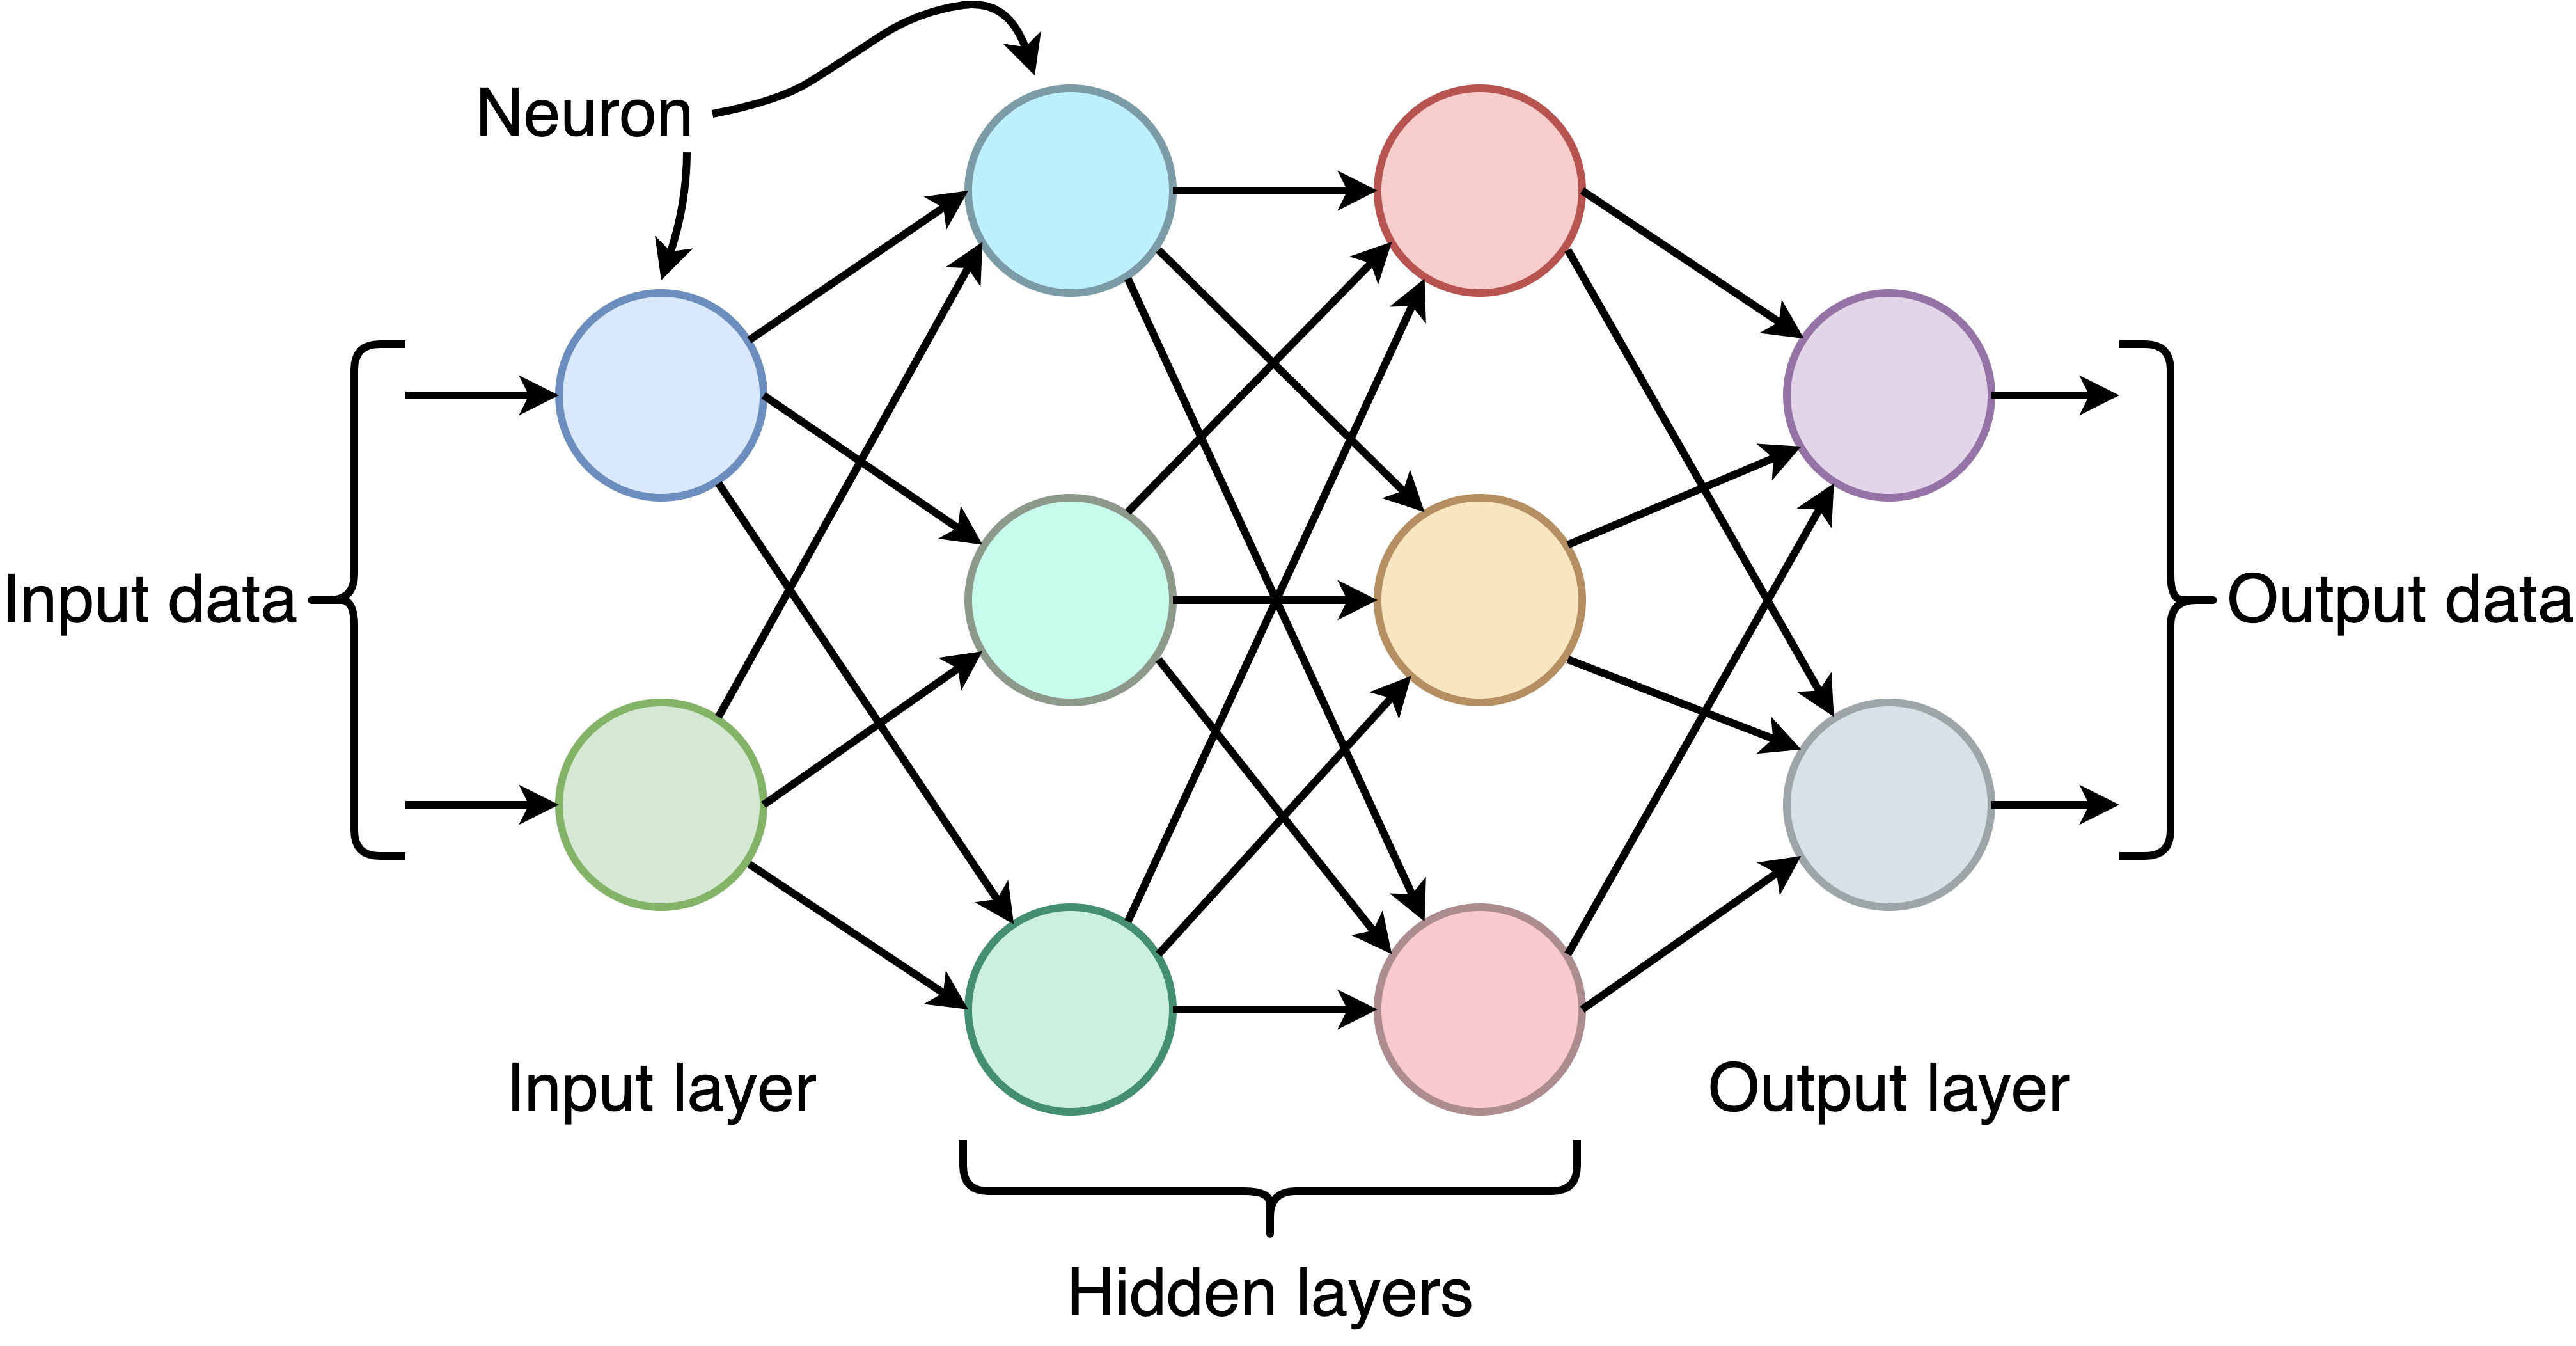
\includegraphics[width=\linewidth]{images/deep_neural_network.png}
        \caption{A fully connected deep artificial neural network with two hidden layers and two input and output neurons. Figure by the author.}
        \label{fig:deep_network}
    \end{figure}

   
    
    Most \glspl{ann} are feedforward, meaning that data is entered on one side, passed through the network, and produces a result on the other end. These networks are often trained using backpropagation, where the network output is compared to the ground truth, and the difference between the estimated result and the ground truth is used to adjust the network weights to minimize this difference. The backpropagation technique is also inspired by biological backpropagation, which occurs when a neuron generates an action potential that sends a voltage spike back to the dendrites. Other methods are proposed instead of feedforward combined with backpropagation, such as the proposed forward-forward algorithm by Hinton \cite{hintonForwardForwardAlgorithmPreliminary2022}.


    Deep neural networks have achieved remarkable achievements, mainly due to their ability to learn from structured and unstructured data, allowing them to learn and generalize knowledge given sufficient amounts and high-quality data \cite{willeminkPreparingMedicalImaging2020}. Before computing power allowed deep networks, hand-made feature extractors were commonly used, using human-predefined features such as texture, shape, and color for object recognition tasks. However, when deep learning was first used in the \gls{imagenet} competition \cite{russakovskyImageNetLargeScale2015}, which is a competition identifying objects from the ImageNet dataset \cite{russakovskyImageNetLargeScale2015}, it achieved great results as shown in Figure \ref{fig:imagenet_results_graph}. This figure shows the methods and their classification error for each year the competition was arranged. It is clear that deep learning made significant strides in 2012 with AlexNet, which was proposed by Krizhevsky et al. \cite{krizhevskyImageNetClassificationDeep2017}. These methods have improved significantly since then, largely thanks to improved methods and hardware. In 2015, deep learning even surpassed the human ability to classify images in ImageNet with the ResNet model proposed by He et al. \cite{heDeepResidualLearning2015, heDelvingDeepRectifiers2015}.
    
    \begin{figure}[htb]
        \centering
        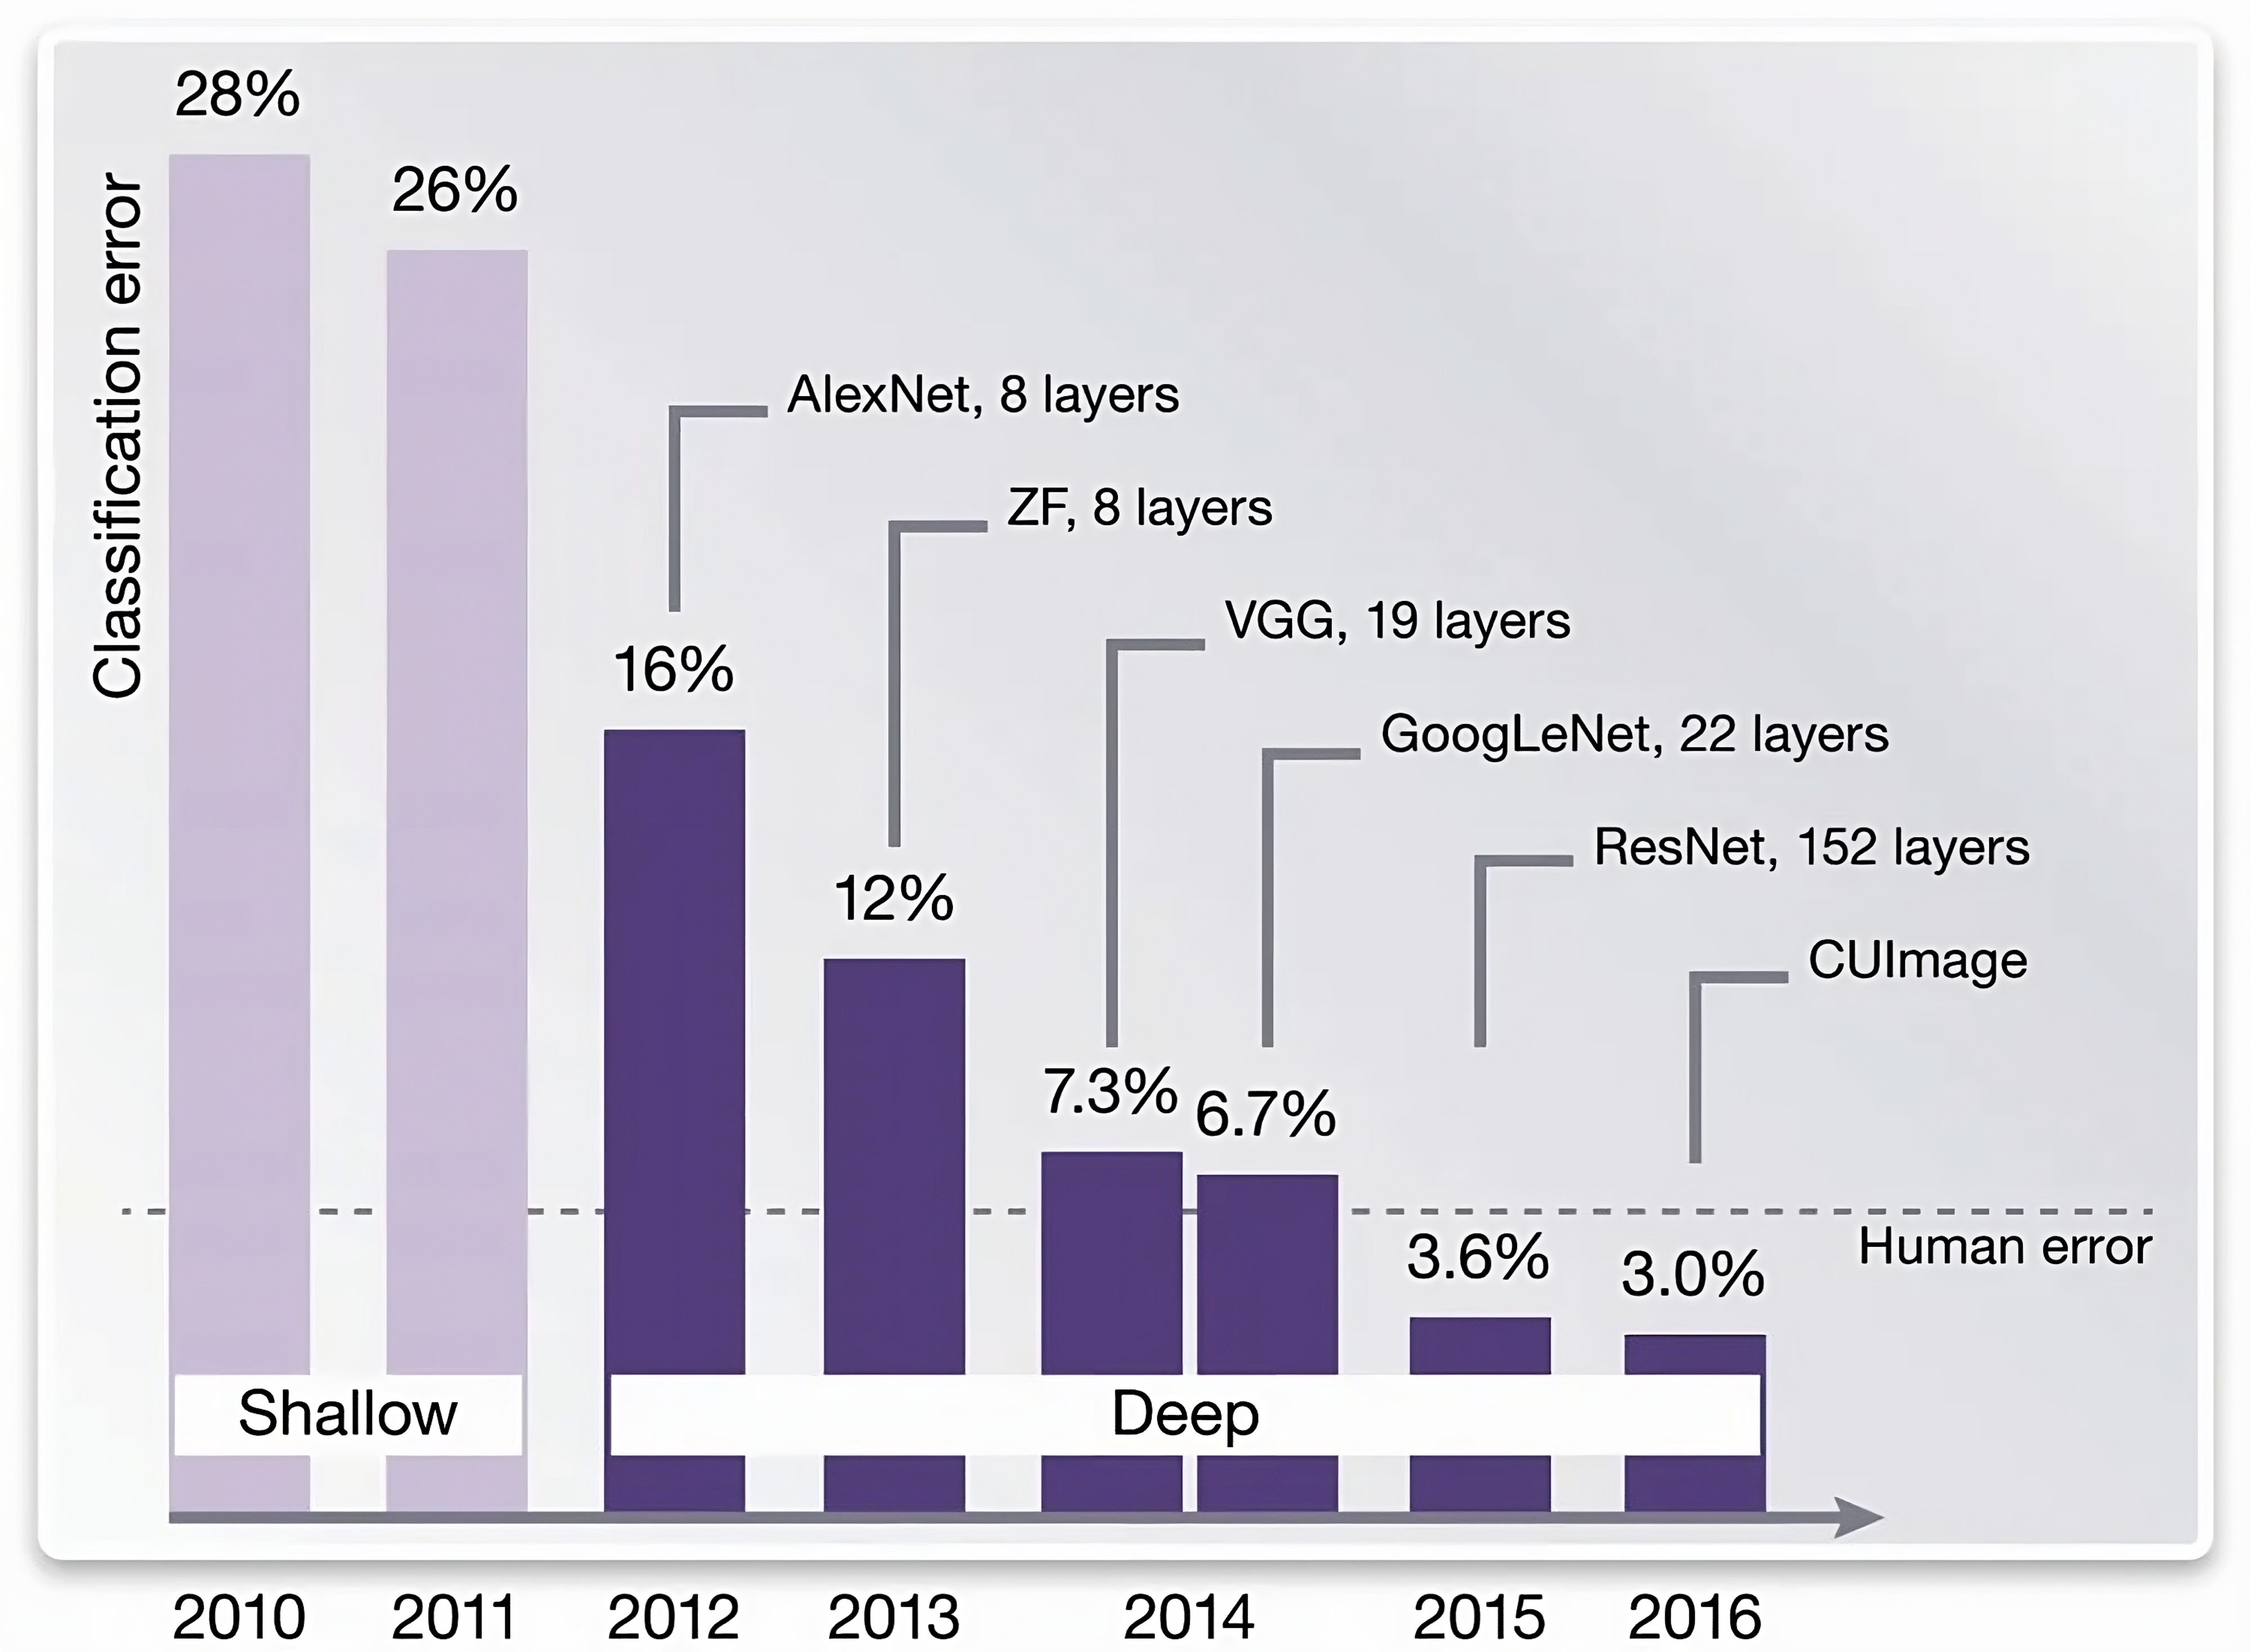
\includegraphics[width=\linewidth]{images/imagenet_results_graph.jpeg}
        \caption[Overview of the ImageNet competition winners from 2010 to 2016.]{Overview of the ImageNet competition winners from 2010 to 2016. The figure shows how deep networks have significantly improved the networks' ability to guess the right label for the images in the ImageNet dataset. In 2015, the deep network ResNet \cite{heDeepResidualLearning2015} surpassed the average human ability to label these images correctly. \\
        Figure credit: Gordon Cooper \cite{cooperSoftwareFrameworkRequirements2017}.}
        \label{fig:imagenet_results_graph}
    \end{figure}


    
    \subsection{Convolutional Neural Networks}

    % Intro to CNNs
    Inspired by biology alongside regular neural networks, the computer vision method called \glspl{cnn} is designed to mimic how the brain's visual cortex processes visual information. \gls{cnn} builds on the idea and technique of neural networks and adds at least one convolutional layer. A convolutional layer allows information about neighboring entities to be obtained from the previous layer. The method has proven particularly effective in computer vision to process and analyze images and video because it can gather context from nearby areas where the convolution is centered. This can help the method extract contextual and semantic relationships that would otherwise have been lost. Both of the proposed methods presented in this thesis use a \gls{cnn}, namely a VGG16 model \cite{simonyanVeryDeepConvolutional2015}, to classify images and extract image features. Therefore, understanding how \glspl{cnn} are constructed and their advantages and uses is relevant.

    % Intro to convolution layers
    The convolution layer works by scanning small filters across the input image, computing dot products between the filter and the image pixels at each location, and creating a feature map. A convolution layer can be considered a flashlight beam aimed at an image. Because of the beam of light, the viewer can see areas of the image that are in the perimeter of the area at which the center of the beam is directed. As the beam of light moves across the image, the viewer understands more of what is in the image. An illustration of a convolution is shown in Figure \ref{fig:convolutuon}.

    \begin{figure}[htb]
        \centering
        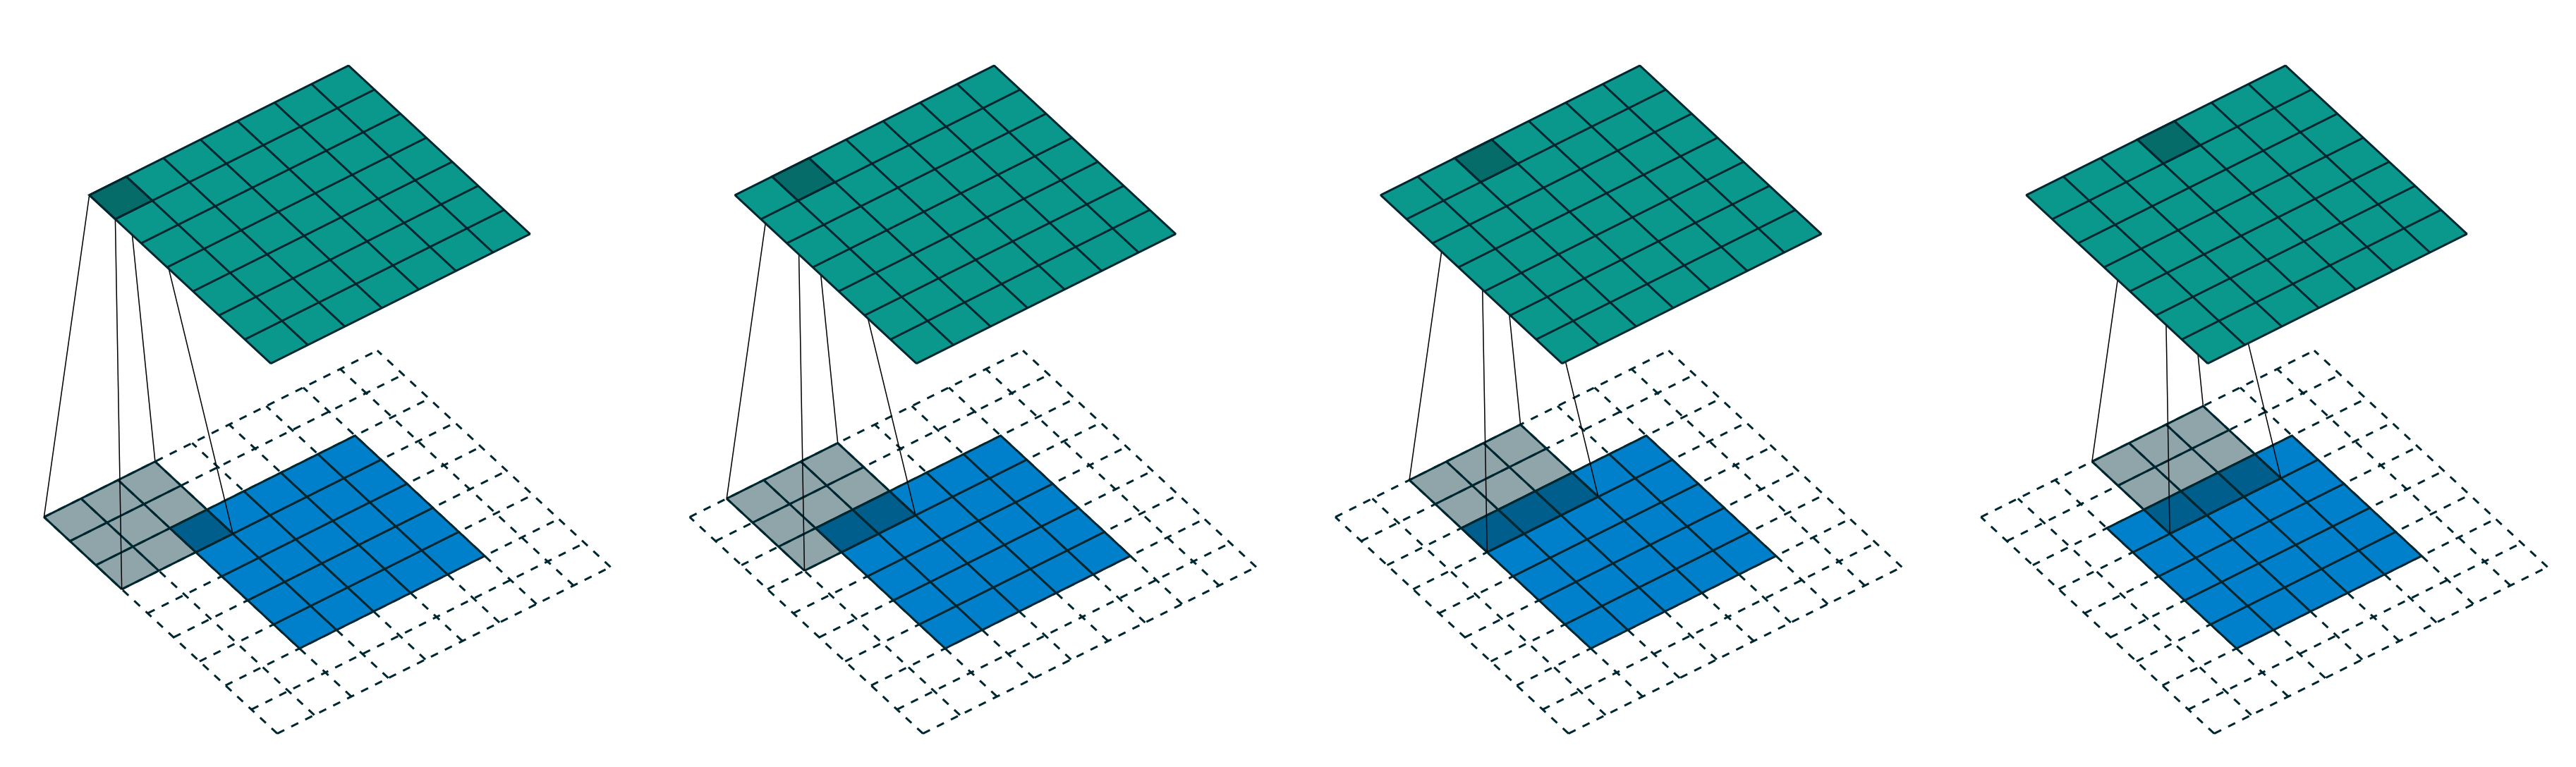
\includegraphics[width=\linewidth]{images/convolution.png}
        \caption[Illustration of a convolution.]{An illustration of a convolution where a $3 \times 3$ kernel is convolved with a $5 \times 5$ input matrix. The convolution illustrated has full padding and a one-step stride.\\
        Figure credit: Vincent Dumoulin and Francesco Visin \cite{dumoulinGuideConvolutionArithmetic2018}.}
        \label{fig:convolutuon}
    \end{figure}


    % Short history and advantage.
    The first \gls{cnn} that trained with backpropagation was first proposed by LeCun et al. in 1989 \cite{lecunHandwrittenDigitRecognition1989} and has since had a huge importance in making machines interpret images and videos. A major advantage of using a convolutional layer is that it can compress information while preserving information and the context around the retrieved information. A very common \gls{cnn} architecture is shown in Figure \ref{fig:vgg_cnn} to see. Also seen in the figure is that a typical \gls{cnn} has a fully connected neural network. A \gls{cnn} often uses fully connected layers, unlike a normal neural network, because of the condensation of information with surrounding information, allowing for a network that can take advantage of using many parameters without overfitting.  

    \begin{figure}[htb]
        \centerline{
        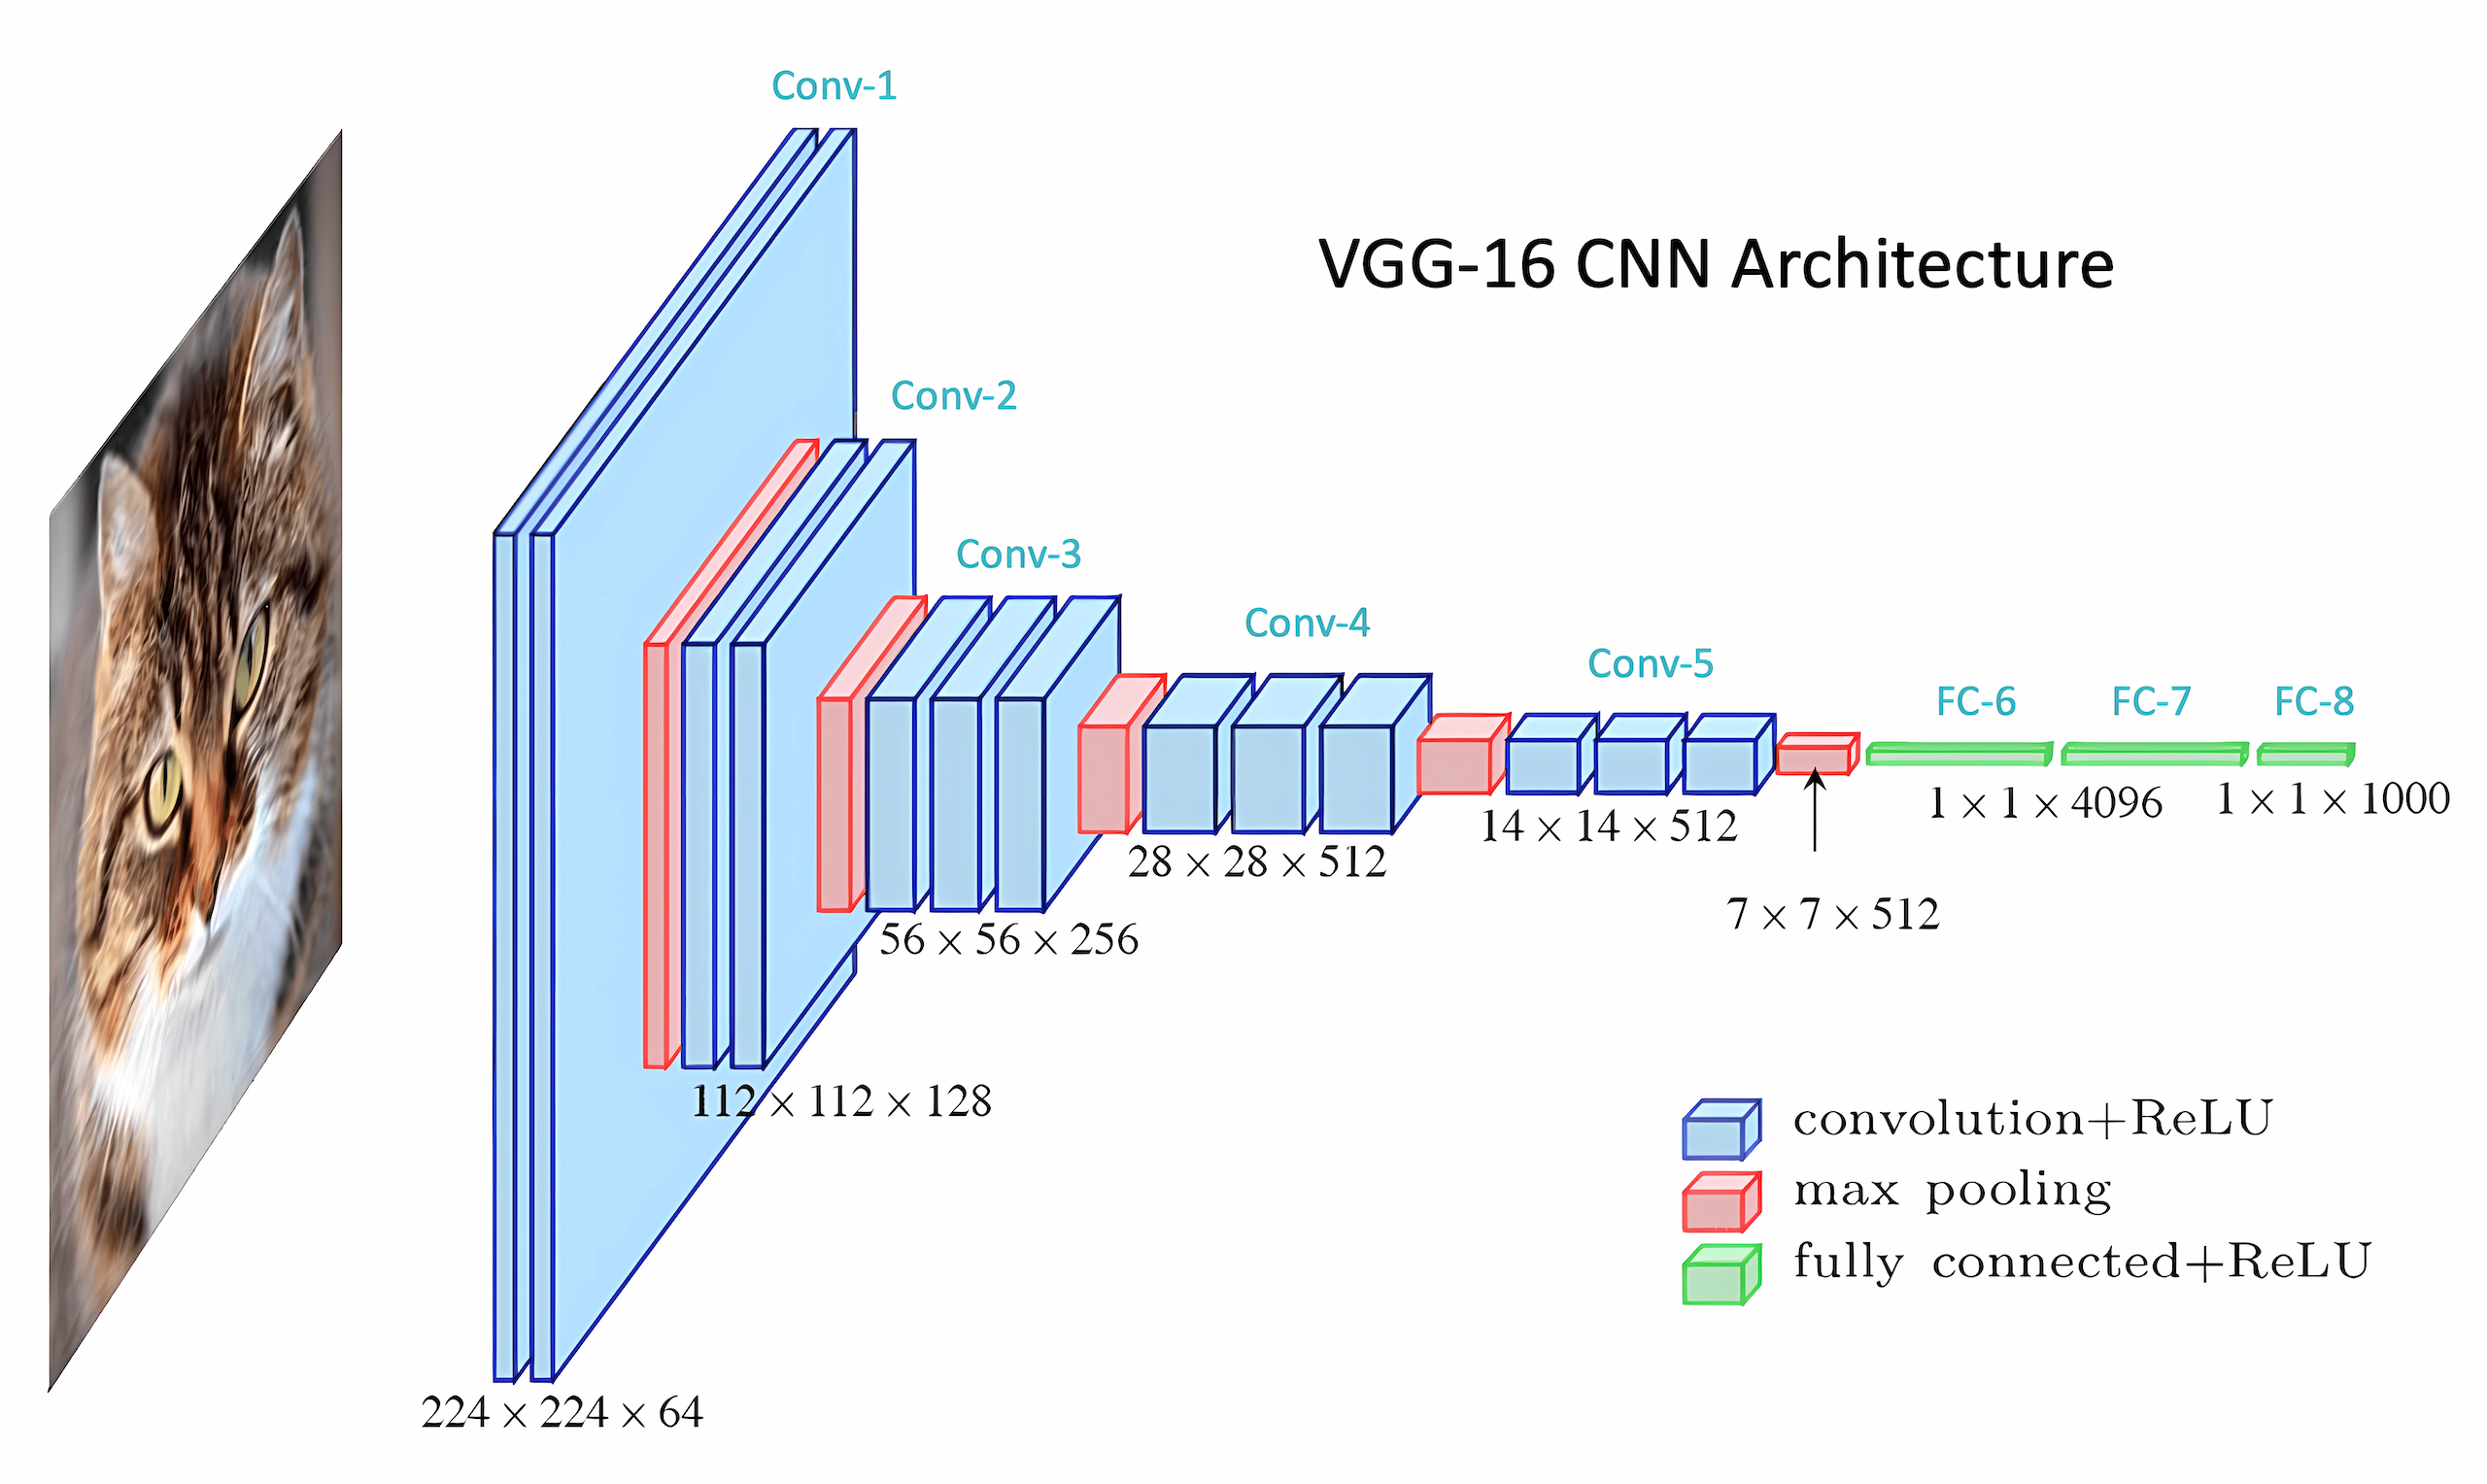
\includegraphics[width=1.1\linewidth]{images/vgg_cnn.png}}
        \caption[Example of a CNN architecture, illustrated by the VGG16 model.]{Example of a typical CNN architecture, here illustrated by the VGG16 model proposed by Simonyan and Zisserman \cite{simonyanVeryDeepConvolutional2015}. As seen in this figure, the first part of the network convolves the input image and extracts feature maps. These feature maps are then fed into a fully connected artificial network that classifies the image in a given class.\\
        Figure credit: Satya Mallick \cite{UnderstandingConvolutionalNeural2023}.}
        \label{fig:vgg_cnn}
    \end{figure}
    
    The convolution layers can be applied to an input image as a series of filters, producing a series of feature maps that emphasize different aspects of the image. These filters have weights that are learned and adjusted during training and are able to recognize different types of patterns of increasing complexity and abstraction from the input image. The training process is similar to regular neural networks and typically updates weights using backpropagation to minimize the loss function and improve the accuracy of the network on the training set. The first layers, closest to the input image, generally recognize low-level features such as edges, lines, corners, texture, and color. As the convolutional layers process the input information, more complex features can be detected that build an abstraction on the information extracted from earlier layers. Convolution layers farther from the image can recognize more high-level features such as shapes, objects, and scenes. Overall, the convolutional layers allow the features of the input image to be analyzed hierarchically, with the early layers capturing low-level features and the later layers capturing high-level features.
    
    % More in-depth architecture with pooling layers.
    \glspl{cnn} are typically designed with multiple layers, similar to deep neural networks, and the last layers are typically fully connected. The fully connected layers take the output of the convolution layers, a set of feature maps, and convert them into a single vector of class scores that represent the probability that the input image belongs to each possible class. The main function of pooling layers in \glspl{cnn} is to reduce the spatial dimensions of the feature maps generated by convolutional layers while preserving the most salient features of the input image. Pooling layers operate on small regions (e.g., 2x2 or 3x3) of the feature maps generated by the previous convolution layers and reduce their size by applying a pooling function, such as max pooling or average pooling, on each region. Max pooling selects the maximum value within each region as the representative value, while average pooling calculates the mean of the region. These operations effectively downsample the feature maps and help reduce the network's sensitivity to small spatial translations and variations in the input. Pooling layers can be inserted after one or more convolutional layers in a \gls{cnn}, and their hyperparameters, such as the size of the pooling area and the stride (i.e., the amount of movement of the pooling window), can be tuned to control the amount of downsampling and the size of the resulting feature maps.
    
    Additionally, pooling layers can prevent network overfitting by reducing the number of parameters and the computation time required for training. The role of pooling layers in \glspl{cnn} is not limited to downsampling. However, they can also help to capture translation invariance, i.e., the property that the learned features are invariant to small translations in the input. The translation invariance is achieved because the max or average operation selects the most prominent feature in a given region, regardless of its exact position. This property allows the network to collect more general relationships in the input data, providing a more general understanding of the network. The overall benefits of pooling layers lie in reducing the spatial dimensions of feature maps while preserving their salient features, resulting in more efficient and robust image analysis.
    
    % Summary
    In essence, the different layers of a \gls{cnn} work together to extract and classify features in images and videos. This makes \glspl{cnn} particularly effective for tasks such as image classification, object detection, and segmentation, where detecting and locating different features of an image is critical for accurate performance. \glspl{cnn} have proven highly effective in image classification tasks, outperforming other types of neural networks and traditional machine learning algorithms. They have been used in various applications, including object recognition, facial recognition, and medical image analysis. With the development of larger and more complex networks and the availability of powerful hardware and software, \glspl{cnn} remains an active area of research and development in machine learning.


\section{Image Captioning}

    The methods proposed in this thesis use techniques to extract information from input images and present a text output. The method to make a model give a textual description to an image is often called image captioning.
    Image captioning is a field of research where the objective is to generate textual descriptions using natural language from the content of an image. This process uses computer vision and \gls{nlp} to gather information from images and give a text that describes or analyzes the image's content. Image captioning is, therefore, a multimodal method that has excelled with the advancements in computer vision, helped considerably by \glspl{cnn} and language models. The motivation for developing this field of research is that its advancements can be utilized in many applications. Image captioning can contribute to improving accessibility for the visually impaired, enhancing search and retrieval systems, assisting in indexing images and video, and making models that can use the combined information in both language and vision to gather information. 

    Image annotation methods typically include modern deep learning techniques, using \glspl{cnn} to extract image features and \glspl{rnn}, typically \glspl{lstm}, to use these extracted image features to generate image captions. \glspl{rnn} are a class of neural networks designed to work on data sequences, like natural language. \glspl{lstm} in particular are designed to combat the problem of vanishing gradients, making them better suited for longer sequences of data. An advantage of the multimodal nature of image labeling methods is that the \gls{cnn} are able to capture spatial features within a given image. In contrast, the \gls{rnn} can structure this information by including temporal dynamics and syntaxes using natural language to create a description that matches the image.


    \section{Attention Mechanisms}
    % Attention is all you need
    The method of attention in modern models was proposed by Bahdanau et al. \cite{bahdanauNeuralMachineTranslation2016} and is a technique that allows the model to search for the most relevant information located in different positions in a sequence. Recent advances in image captioning have seen the use of attention mechanisms, both in the vision and language modalities. Attention mechanisms have allowed the model to selectively focus on different parts of the image when generating captions. By selectively paying attention to different areas of the image, the model is able to capture the fine-grained details needed to generate accurate and descriptive captions. This has significantly improved the quality of captions, where attention-based methods often outperform traditional non-attention-based techniques \cite{liEntangledTransformerImage2019}. 
    
    The attention technique is motivated by nature and is inspired by cognitive attention mechanisms. The main advantage is that the attention allows the method to highlight some parts of the input data while giving other, less important parts a lower priority. Attention mechanisms aim to carefully learn which parts of the data are most important in context and prioritize those parts.


    % One attention method that has made huge advancements is the Transformer architecture proposed by Vaswani et al. The Transformer differs from a traditional network in that it entirely dispenses recurrence and convolutions. Instead, it is solely based on the attention mechanism, using self-attention and point-wise, fully connected layers for both the encoder and decoder of the architecture. 

    Attention-like mechanisms have been part of the research field of machine learning since the 1990s. Initially, it was introduced under names like sigma pi units, multiplicative modules, and hyper-networks \cite{lecunRNNsGRUsLSTMs2020}. The flexibility of attention-based techniques comes from their ability to learn which parts of the input data are most important in context. Attention can be implemented in different approaches, where the most notable are global, local, soft, and hard attention. Global and local determine if all the weights in the hidden states of the encoder should be used or a local subset. Global attention could become computationally expensive and use redundant weights; therefore, local is often used. Hard and soft attention determines how a hidden state gets calculated. Hard attention uses the attention scores, whereas soft attention uses a weighted sum of the hidden states in the encoder. Using the soft attention method, the model can change focus during runtime, which can have a major advantage compared to non-attention models, which remain unchanged during inference. The ability to adaptively prioritize input data has popularized attention-based models in natural language processing, multimodal, and multisensory computing. Some effective methods that use attention are \glspl{lstm}, Transformers, and Perceivers \cite{hochreiterLongShorttermMemory1997, vaswaniAttentionAllYou2017, jaeglePerceiverGeneralPerception2021}. An overview of the Transformer model proposed by Vaswani et al. \cite{vaswaniAttentionAllYou2017} can be seen in Figure \ref{fig:transformer_architecture}. The use of autoregressive transformers and attention mechanisms have made it possible to make large language models, such as \gls{bert}, \gls{bart}, and \gls{gpt} \cite{devlinBERTPretrainingDeep2019, lewisBARTDenoisingSequencetoSequence2019, radfordImprovingLanguageUnderstanding2018, radfordLanguageModelsAre2019, brownLanguageModelsAre2020, openaiGPT4TechnicalReport2023}. 


    \begin{figure}[htb]
        \centering
        \centerline{
        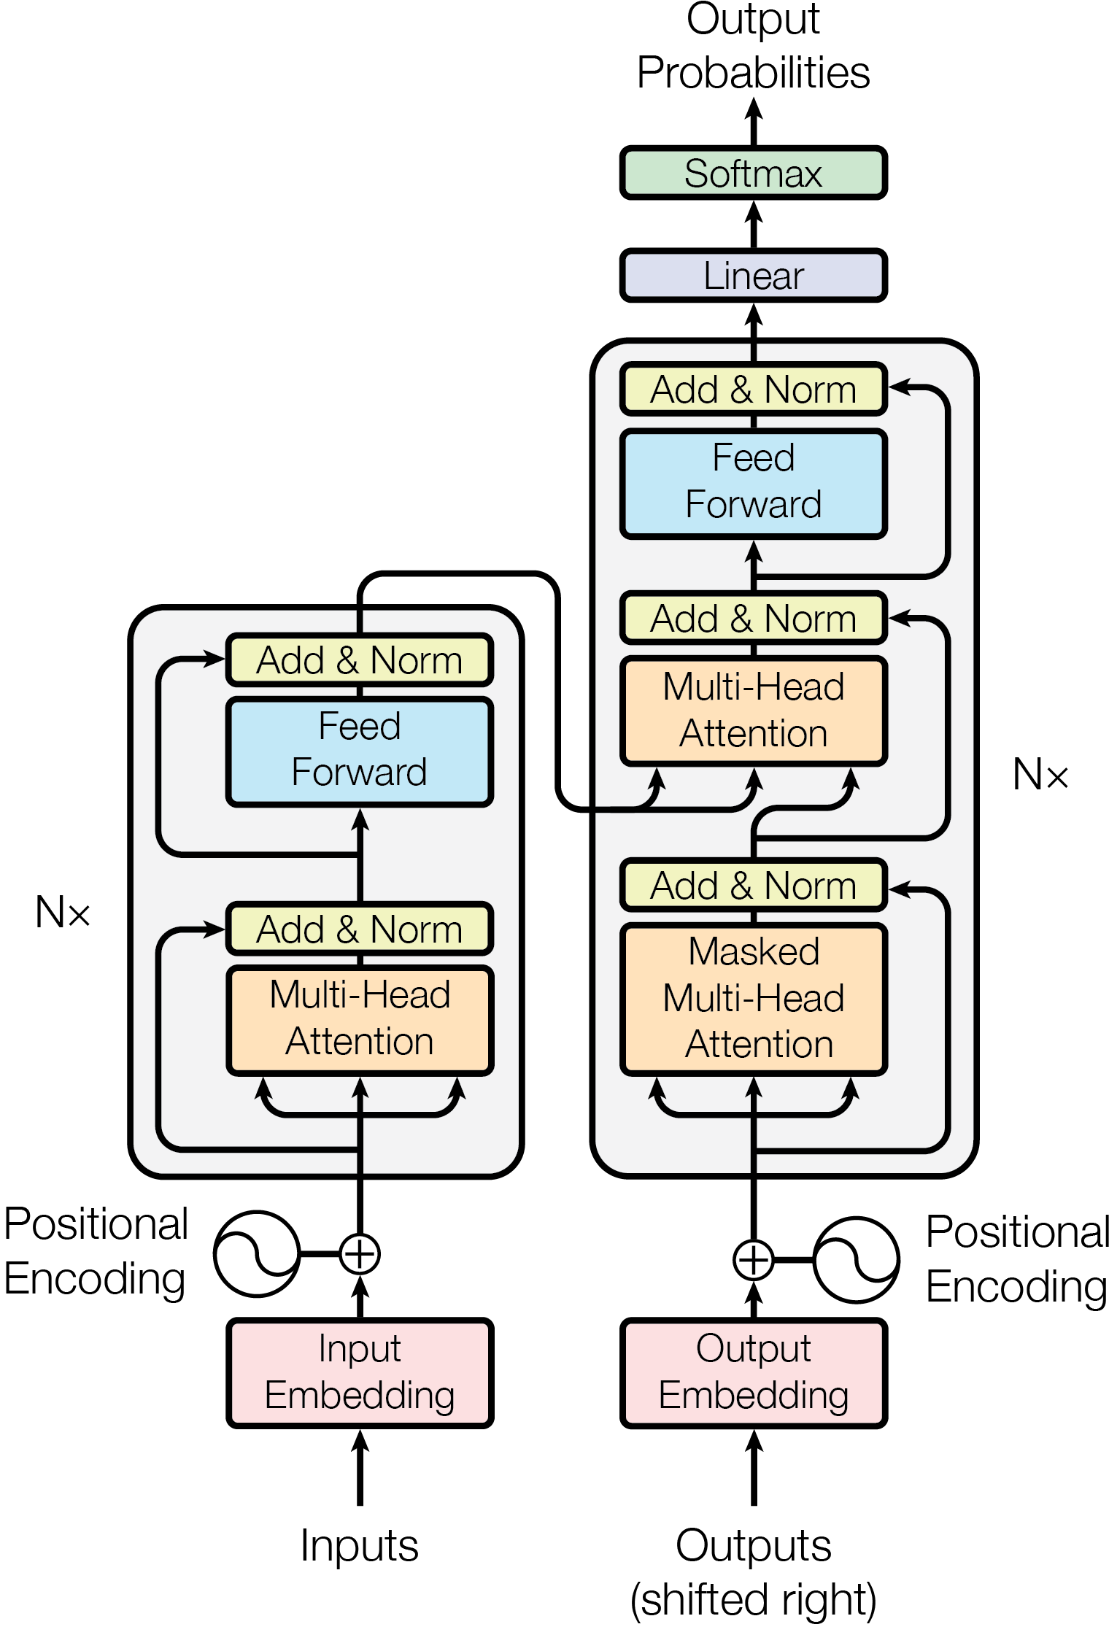
\includegraphics[width=10cm]{images/Transformer_architecture.png}}
        \caption[Transformer architecture proposed by Vaswani et al.]{Transformer architecture proposed by Vaswani et al.\\
        Figure credit: Vaswani et al. \cite{vaswaniAttentionAllYou2017}.}
        \label{fig:transformer_architecture}
    \end{figure}
    
    In the language part of the model, the attention mechanisms can also be used to selectively focus on a different part of the features extracted from the image. They can therefore generate the textual context that is most relevant to identify contents in the image correctly. This way, the model can describe the essential features of the picture or video using natural language. Some recent models have moved from CNN architectures to extract image features and solely rely on attention mechanisms to gather relevant information in the visual domain. Some of these models are \gls{vit}, alongside versions of \gls{bert} that incorporate vision, like ViBert \cite{leiLessMoreClipBERT2021, liVisualBERTSimplePerformant2019, suVLBERTPretrainingGeneric2020}. % An image is worth 16x16 words: Transformers for image recognition at scale, ViBert 

    
    Attention weights are most commonly learned during training through backpropagation and gradient descent. The weights are used to give relevance scores to different words in context for being the following word in the text sequence. Attention can be derived in several ways, notably global vs. local and soft vs. hard. Global and local attention refers to different ways of weighting input features, where a global process weights all input features equally without prioritizing specific parts. Each input feature is considered when computing the output.
    In contrast, local attention refers to a more selective process in which the input features are weighted differently and are therefore prioritized when computing the output. This prioritized subset is usually determined by a region or window around the previous output or target position, borrowing ideas from how \glspl{cnn} retrieves surrounding data from an image.
    
    Soft and hard attention refers to the different methods of incorporating attention into a neural network. Soft attention is computed by a weighted average of the input features, with the weights learned during training and typically normalized to a value between 0 and 1. This weighting allows the model to consider multiple input parts simultaneously, gathering information from a more extensive range. On the other hand, hard attention selects a particular input feature to take care of at each time step, effectively forcing the model to make a discrete decision. This attention implementation can make the model less flexible but excel when the input is highly structured and easily segmented into distinct parts.


    
    %\subsection{Image Classification}


    %\subsection{Natural Language Processing}




% \section{Visual Question Answering}
    % What is VQA

    % Why is VQA important and interesting
    




\section{Model evaluation}
    In the field of machine learning and artificial intelligence, model evaluation refers to the process of measuring the quality and effectiveness of a trained model. These evaluations are essential in developing machine learning systems, allowing researchers and practitioners to determine their models' accuracy and generalization performance. Model evaluation helps to identify any weaknesses or shortcomings in a model's design or training process and enables researchers to make improvements to enhance the model's performance.

    \subsection*{Performance Metrics}
    Performance metrics are integral to machine learning models, allowing us to measure how well a model performs on a given task. These metrics evaluate the accuracy and effectiveness of a model's predictions by comparing them to the actual values. The choice of performance metrics depends on the problem being solved and the type of model being used. For example, in a binary classification problem, the model's accuracy can be used as a performance metric. In contrast, for multi-class classification problems, metrics like precision, recall, and $F1$ score are more appropriate. In general, model evaluation metrics like precision and recall provide information about the performance of a model on a particular class, while accuracy and $F1$ score provide an overall measure of model performance. Choosing appropriate performance metrics when developing a machine learning model is essential to ensure that the model's predictions align with the intended use case.
    
     % Precision and  Recall
    \subsection{Precision and Recall}
    Precision and recall are two important metrics used in classification tasks to evaluate the performance of a model. 
    Both precision and recall are based on the values in the confusion matrix, which is a table that summarizes the performance of a classification model. The confusion matrix contains four values: true positives, false positives, true negatives, and false negatives. True positives and false positives correspond to the model's positive predictions, while true negatives and false negatives correspond to the negative predictions. Figure \ref{fig:confusion_matrices} shows an example of a confusion matrix. The precision and recall are defined as follows.
        

    \begin{itemize}
        \item Precision: the ratio of correct answers among all answers proposed by the model, and it measures how precise the model's positive predictions are. The precision score can be calculated as follows:
        
        \begin{equation}
            \text{Precision} = \frac{\text{True Positive}}{\text{True Positive} + \text{False Positive}}
        \end{equation}
        
        \item Recall: the ratio of correct answers proposed by the model among all possible correct answers, and it measures how well the model is able to identify positive instances. The recall score can be calculated as follows:

        \begin{equation}
            \text{Recall} = \frac{\text{True Positive}}{\text{True Positive} + \text{False Negative}}
        \end{equation}
    \end{itemize}


    \begin{figure}[htb]
     \centerline{
         \begin{subfigure}[b]{0.5\textwidth}
             \centering
             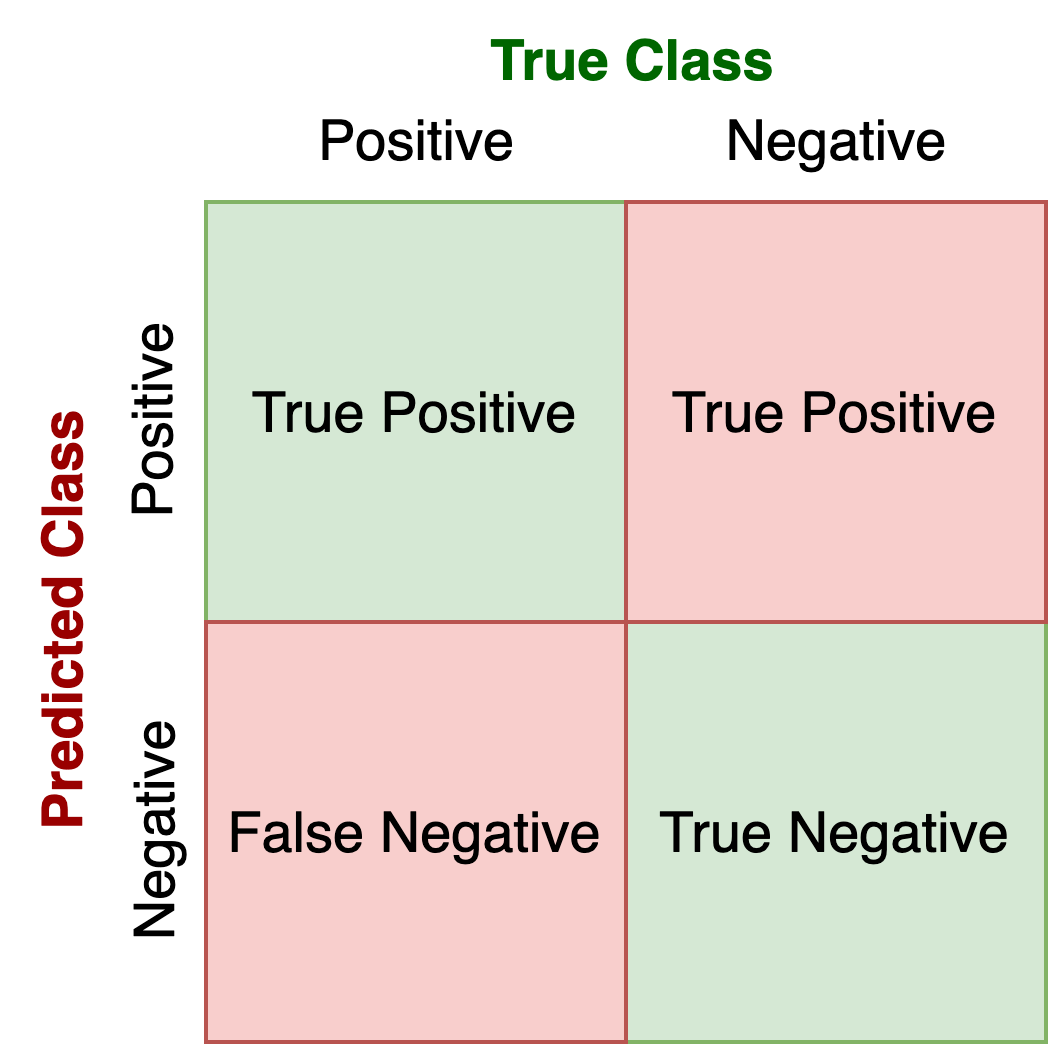
\includegraphics[width=\textwidth]{images/confusion_matrix_binary.png}
             \caption{Example of a confusion matrix of a binary classifier. A perfect classifier would have just true predictions.}
             \label{fig:confusion_binary}
         \end{subfigure}
         \hspace{0.1\textwidth}
         \begin{subfigure}[b]{0.5\textwidth}
             \centering
             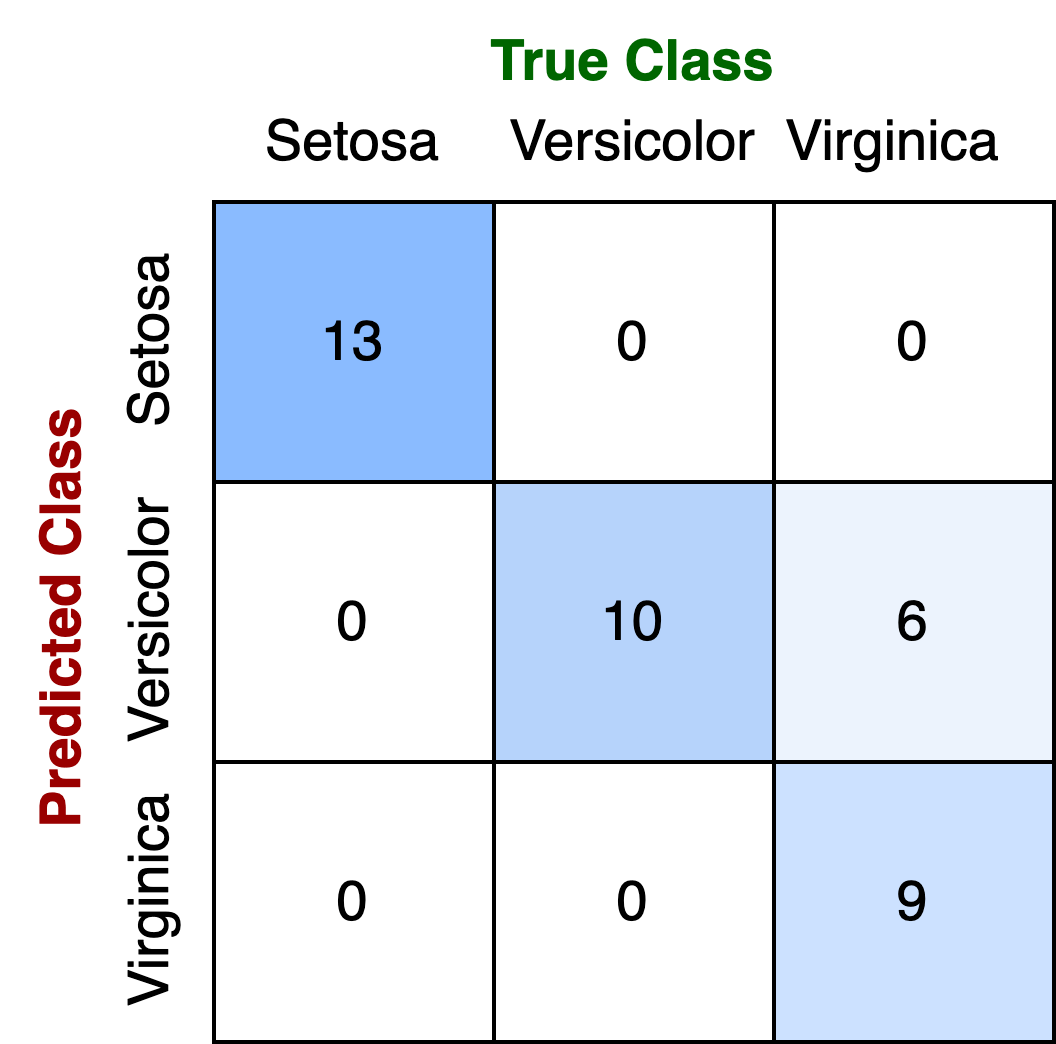
\includegraphics[width=\textwidth]{images/confusion_matrix_multi.png}
             \caption{Example of a confusion matrix of a multi-class classifier. An adapted example from scikit-learn \cite{ConfusionMatrix}.}
             \label{fig:confusion_multi}
         \end{subfigure}
         }
        \caption{Example of confusion matrices, both for a binary (a) and multi-class (b) classifier. Figure by the author.}
        \label{fig:confusion_matrices}
    \end{figure}


    % Accuracy
    \subsection{Accuracy}
\begin{comment}
https://www.statology.org/f1-score-vs-accuracy/
Accuracy:

Pro: Easy to interpret. If we say that a model is 90% accurate, we know that it correctly classified 90% of observations.

Con: Does not take into account how the data is distributed. For example, suppose 90% of all players do not get drafted into the NBA. If we have a model that simply predicts every player to not get drafted, the model would correctly predict the outcome for 90% of the players. This value seems high, but the model is actually unable to correctly predict any player who gets drafted.
\end{comment}
    Accuracy is a commonly used evaluation metric in statistics and artificial intelligence for classification models. It is a metric that is easy to interpret by humans because it measures the percentage of correctly predicted labels out of all the predictions made by the model. Accuracy is a valuable metric when the classes in the dataset are balanced, meaning that the number of instances for each class is roughly equal. However, when the classes are imbalanced, accuracy can be misleading. For instance, in a dataset with 95\% of the samples belonging to class A and only 5\% belonging to class B, a model that always predicts class A will have an accuracy of 95\% but will not be helpful in practice if the real-world data does not have the same distribution.

    Moreover, accuracy does not account for false positives and false negatives, as seen in Formula \ref{eq:accuracy}. False positives occur when the model predicts a positive label for a sample that is negative, while false negatives occur when the model predicts a negative label for a sample that is positive. In some applications, such as medical diagnosis, false negatives may be more costly than false positives, and accuracy alone may not be an adequate metric for evaluating model performance. Therefore accuracy can be a helpful and easily understandable metric when there is no critical downside predicting false negatives and the classes in the dataset are balanced. When dealing with real-world datasets, the classes are often not balanced, and a more suitable metric can be the $F_1$ score.
    


    \begin{equation}
        \text{Accuracy} = \frac{\text{True Positive} + \text{True Negative}}{\text{Total Sample Size}}
        \label{eq:accuracy}
    \end{equation}


    % F1 score
    \subsection{F\textsubscript{1} score}


    The $F_1$ score is a statistical metric used to measure a model's performance on a dataset. It evaluates the performance of a binary classifier, which is a classification system that makes predictions for two possible classes, for example, positive and negative. The $F_1$ score can be calculated using the formula in Equation \ref{eq:f1}.

    \begin{equation}
        F_1 = 2 \frac{\text{Precision} \cdot \text{Recall}}{\text{Precision} + \text{Recall}}
        \label{eq:f1}
    \end{equation}

    In the context of question answering by a large language model, the $F_1$ score can be used to evaluate the accuracy of the model's responses to questions. Specifically, the score measures the harmonic mean of the model's precision and recall.

    \begin{comment}
https://www.statology.org/f1-score-vs-accuracy/
F1 Score:

Pro: Takes into account how the data is distributed. For example, if the data is highly imbalanced (e.g. 90% of all players do not get drafted and 10% do get drafted) then F1 score will provide a better assessment of model performance.

Con: Harder to interpret. The F1 score is a blend of the precision and recall of the model, which makes it a bit harder to interpret.

As a rule of thumb:

We often use accuracy when the classes are balanced and there is no major downside to predicting false negatives.

We often use F1 score when the classes are imbalanced and there is a serious downside to predicting false negatives.
    \end{comment}


    \subsection{Perplexity}

    Perplexity, often referred to as PPL, is one of the most common metrics for evaluating language models. In information theory, perplexity measures how well a probability distribution or model predicts a sample. Intuitively, perplexity means being surprised, and in practice, it measures how surprised the model is when it sees new data. The lower the perplexity score, the better the training. Perplexity is usually only used to determine how well a model has learned the training set. 

    At its core, a language model is a probability distribution over a set of words, known as the model vocabulary. Considering all of its previous words, the model indicates the probability that a given word will appear in the vocabulary. Usually, the word with the maximum likelihood is selected as the next predicted word in the sequence.

    As an evaluation metric, perplexity can be used to compare probabilistic models, and low perplexity indicates that the probability distribution is good at predicting the sample. This probability can be calculated by multiplying a sequence of conditional probabilities for each word by its previous words, which indicates the probability of this sequence.
    Given a tokenized sequence $X = (x_0, x_1, ..., x_t)$, the perplexity of the sequence \textit{X} is given in the Formula \ref{eq:2_perplexity}.
        

    \begin{equation}
    \operatorname{Perplexity}(X)=\exp \left\{-\frac{1}{t} \sum_i^t \log p_\theta\left(x_i \mid x_{<i}\right)\right\}
    \label{eq:2_perplexity}
    \end{equation}

    In this formula, $\log p_\theta\left(x_i \mid x_{<i}\right)$ is the log-likelihood for the token with index $i$, given the previous tokens $x_{<i}$.

\section{Frameworks}
    %\subsection{PyTorch}
    This section briefly describes the most important external frameworks used in this thesis.
    
    \subsection{TensorFlow}
    
    TensorFlow is the framework used in the FLEX-VQA method proposed in this thesis. Here the framework is used to train the FLEX model to find connections between images and captions. A more detailed description of the implementation is discussed in Chapter \ref{sec3:flex_vqa}.

    
    TensorFlow is an open-source machine learning framework developed and maintained by the Google Brain team. It was first introduced in 2015 and has since become one of the most widely used frameworks in machine learning.
    TensorFlow's core strength lies in its ability to handle large-scale machine learning models easily. It provides a highly optimized execution engine that efficiently computes complex models. This optimization is achieved through dataflow graphs, representing the computations as a directed graph of nodes and edges. Each node in the graph represents an operation, while the edges represent the data flow between operations. This architecture allows for parallelism and efficient computation, making it an attractive choice for large-scale machine learning tasks.
    
    One of the key advantages of TensorFlow is its versatility. It supports various machine learning tasks, including classification, regression, clustering, and reinforcement learning. It also supports deep learning models, such as \glspl{cnn}, \glspl{rnn}, and transformers.

    
    
    Google has developed a specialized hardware data processor, the Tensor Processing Unit (TPU), an application-specific integrated circuit (ASIC). The TPU is tailored to optimize the TensorFlow framework, functioning as an AI accelerator. By utilizing the TPU rather than a conventional GPU, models can achieve superior optimization while minimizing the time and power consumption required to train and run compatible models. This hardware optimization is not exclusive to TensorFlow, as other processor designers have integrated specialized machine learning chips. The increased prevalence of such chips will enable machine learning to be executed on new devices while reducing the carbon footprint. Although this thesis does not employ such chips, they serve as a noteworthy illustration of the promising prospect of deploying machine learning techniques in energy-efficient devices, ultimately paving the way toward the democratization of \gls{ai}.


    

    \subsection{Text tokenization}

    Large language models such as GPT-3 \cite{brownLanguageModelsAre2020} and BERT \cite{devlinBERTPretrainingDeep2019} are trained on massive amounts of text data and can generate coherent and contextually relevant sentences, paragraphs, and even longer texts. However, feeding raw text data to such models can be computationally expensive and lead to suboptimal results due to high input variability. Therefore, text pre-processing techniques such as tokenization convert raw text into a form the model can more easily process.
    
    Tokenization is the process of splitting text into smaller units, called tokens, such as words, subwords, or characters. These tokens are then assigned a unique integer identifier and are often converted into fixed-length sequences, which can be fed into the language model. This process allows the model to handle text data more efficiently, reduces input variability, and helps to improve the training and inference times.
    
    Using a tokenizer specific to the language model used is crucial because it ensures that the tokens are consistent with the vocabulary and encoding scheme of the model. For example, using a tokenizer that splits words differently than the one used during the pre-training of the model can lead to inconsistencies and decreased performance.
    
    Various tokenization techniques are available, such as byte-pair encoding (BPE), WordPiece, and SentencePiece. BPE is a subword tokenization method that progressively merges the most frequent pairs of characters in a corpus to create a fixed-size vocabulary. WordPiece is a similar technique that uses a predefined list of subword units to tokenize words. SentencePiece is a more flexible method for creating a custom vocabulary that can handle rare and out-of-vocabulary words.
    
    Each of these techniques has its upsides and downsides. BPE and WordPiece are efficient and widely used, but they can result in a large vocabulary size and require additional processing steps to handle out-of-vocabulary words. SentencePiece can manage rare and out-of-vocabulary words better but can be computationally expensive due to their adaptive nature.

    This work uses a tokenizer built on top of SentencePiece, adapted and trained specifically to the language model, namely LLaMA. A more detailed explanation of this tokenizer can be seen later in Chapter \ref{sec2:text_encoding}, which details the implemented method.